\documentclass[12pt,a4paper]{article}
\usepackage[utf8]{}
\usepackage[T1]{fontenc}
\title{EP1200 - Datasys anteckningar}
\author{Yunshan Luo}


\renewcommand{\baselinestretch}{0.2}

\setlength{\hoffset}{-18pt}         
\setlength{\oddsidemargin}{0pt} % Marge gauche sur pages impaires
\setlength{\evensidemargin}{0pt} % Marge gauche sur pages paires
\setlength{\marginparwidth}{54pt} % Largeur de note dans la marge
\setlength{\textwidth}{481pt} % Largeur de la zone de texte (17cm)
\setlength{\voffset}{-18pt} % Bon pour DOS
\setlength{\marginparsep}{7pt} % Séparation de la marge
\setlength{\topmargin}{0pt} % Pas de marge en haut
\setlength{\headheight}{13pt} % Haut de page
\setlength{\headsep}{4pt} % Entre le haut de page et le texte
\setlength{\footskip}{27pt} % Bas de page + séparation
\setlength{\textheight}{720pt} % Hauteur de la zone de texte (25cm)

\usepackage{natbib}
\usepackage{graphicx}
\usepackage{amssymb}
\usepackage{amsmath} % Required for the align* environment
\usepackage{float}
\usepackage{pgfplots} 
\usepackage{algorithm}
\usepackage{algpseudocode} % test comment
\pgfplotsset{compat=1.18}


\begin{document}
\section{Section 1}
\subsection{Boolean logic}
Example of common truth tables: AND, OR, NOT:
\begin{figure}[H]
    \centering
    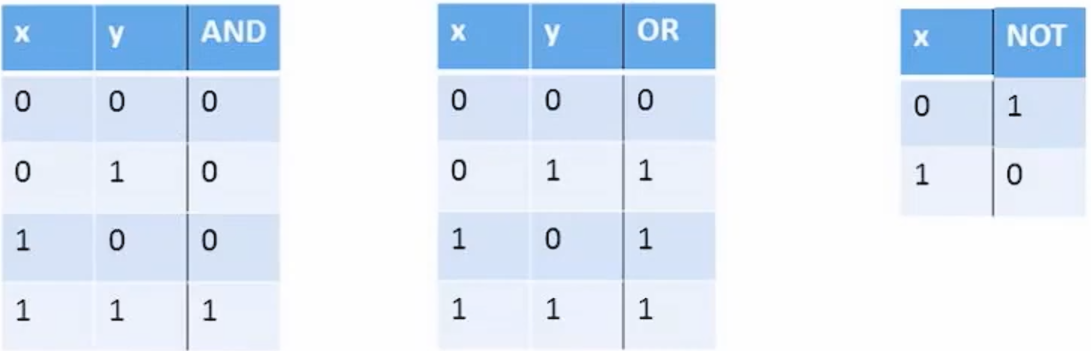
\includegraphics[width=1\textwidth]{truthTable.png}
\end{figure}

\subsection{Evaluating Boolean expressions}
$$\text{NOT(0 OR (1 AND 1)) = NOT(0 OR 1) = NOT(1) = 0}$$

\subsection{Evaluating Boolean functions}
$$\text{f(x,y,z) = (x AND y) OR (NOT(x) AND z)}$$
\noindent We can derive the truth table for this function by evaluating it for all combinations of x, y, and z:
\begin{figure}[H]
    \centering
    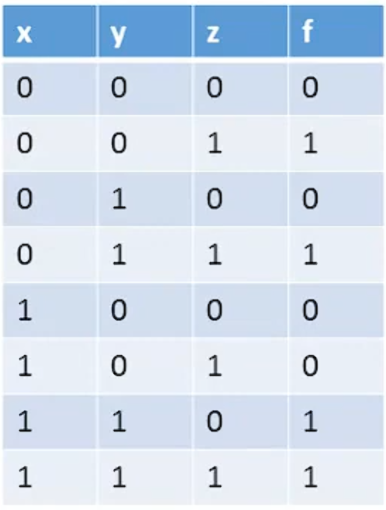
\includegraphics[width=0.5\textwidth]{truthTable2.png}
\end{figure}
\newpage
\subsection{Boolean Identities}
\begin{itemize}
    \item Commutative Laws applies for AND and OR:
    \begin{itemize}
        \item x AND y = y AND x
        \item x OR y = y OR x
    \end{itemize}
    \item Associative Laws applies for AND, OR and NOT:
    \begin{itemize}
        \item (x AND y) AND z = x AND (y AND z)
        \item (x OR y) OR z = x OR (y OR z)
        \item NOT(NOT(x)) = x
    \end{itemize}
    \item De Morgan's Laws describes how NOT interacts with AND and OR:
    \begin{itemize}
        \item NOT(x AND y) = NOT(x) OR NOT(y)
        \item NOT(x OR y) = NOT(x) AND NOT(y)
    \end{itemize}
\end{itemize}

\subsection{Example of applying Boolean identities}
\begin{align*}
        &   \text{NOT(NOT(x) AND NOT(x or y))}: \\
        & = \text{NOT(NOT(x) AND (NOT(x) AND NOT(y)))} \\
        & = \text{NOT(NOT(x) AND NOT(x) AND NOT(y))} \\
        & = \text{NOT(NOT(x) AND NOT(y))} \\
        & = \text{NOT(NOT(x)) OR NOT(NOT(y))} \\
        & = \text{x OR y}
\end{align*}

\subsection{Truth table to Boolean expression}
\begin{enumerate}
    \item Find where function output = 1
    \item Not on all 0s and keep all 1s
    \item And all variables in the same row together
    \item Or all the results of all rows where output = 1
    \item Simplify the expression using Boolean identities
    \item All Boolean functions can be expressed using only AND, or, and NOT
    \item Furthermore, all boolean functions can be expressed as NAND
    \item Proof that all logic can be implemented using only NAND:
    \begin{itemize}
        \item NOT(x) = x NAND x
        \item x AND y = NOT(x NAND y) = (x NAND y) NAND (x NAND y)
        \item x OR y = NOT((NOT(x) NAND NOT(y))) = (x NAND x) NAND (y NAND y)
    \end{itemize}
\end{enumerate}

\subsection{Logic gates}    
\begin{itemize}
    \item Elementary logic gates: AND, OR, NOT, NAND
    \item Composite logic gates: Mux, Adder, Dmux
\end{itemize}

\subsection{Nand gate}
\begin{figure}[H]
    \centering
    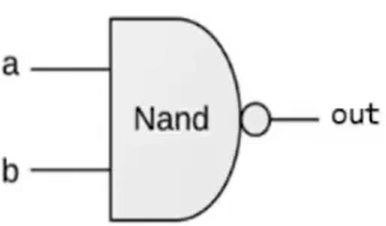
\includegraphics[width=0.5\textwidth]{nand.png}
\end{figure}

Truth table:
\begin{figure}[H]
    \centering
    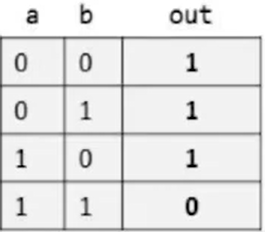
\includegraphics[width=0.3\textwidth]{nandTruthTable.png}
\end{figure}

\subsection{Other gates}
OR gate:
\begin{figure}[H]
    \centering
    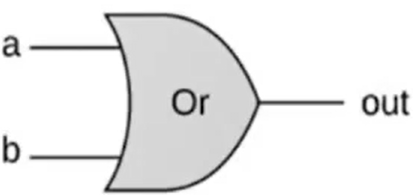
\includegraphics[width=0.5\textwidth]{or.png}
\end{figure}

\noindent NOT gate:
\begin{figure}[H]
    \centering
    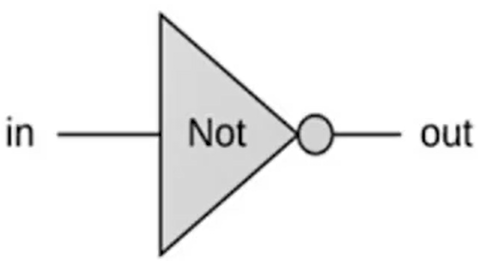
\includegraphics[width=0.5\textwidth]{not.png}
\end{figure}

\subsection{Circuit implementation}
\begin{itemize}
    \item Logic gates can be represented as circuits
    \item For example through parallel and series connections can represent AND and OR
\end{itemize}

\subsection{Hardware Description Language (HDL)}
General idea of building XOR:
out = 1 when:
$$\text{(a and NOT(b)) or (b and NOT(a)) = a XOR b}$$
\begin{figure}[H]
    \centering
    
\includegraphics[width=0.75\textwidth]{xor.png}
\end{figure}

\begin{itemize}
    \item The red connections are those that we make
    \item Each red connections should be named appropriately
    \item The black connections comes with the hardware
    \item The order of the HDL language does not matter
\end{itemize}       

\subsection{Hardware simulation}
Simulation options:
\begin{itemize}
    \item Interactive -- Manually input values and observe output
    \item Script-based -- Running a test script and see if the output matches expected output
    \item Output and compare files -- Running a test script and compare the output file with expected output file
\end{itemize}

\subsection{Multi-bit Buses}
It is easier to think in multiple bits instead of single bits

\subsection{Example: 16-bit adder}
\begin{figure}[H]
    \centering
    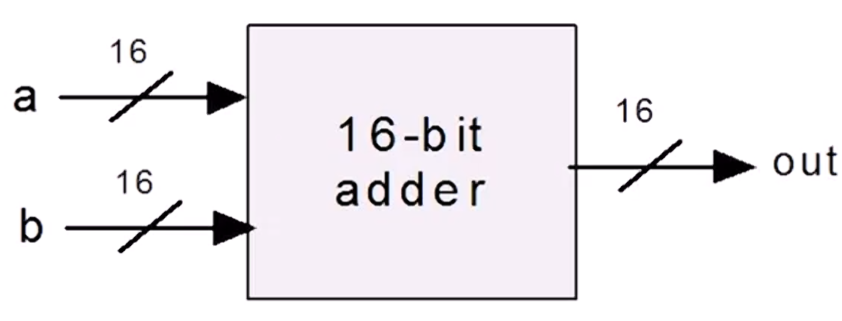
\includegraphics[width=0.5\textwidth]{adder.png}
\end{figure}

\subsection{Multiplexor}
\begin{figure}[H]
    \centering
    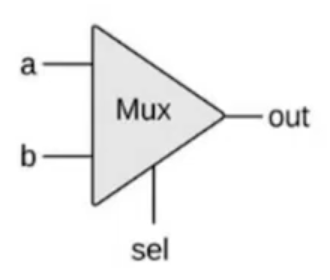
\includegraphics[width=0.5\textwidth]{mux.png}
\end{figure}
$$\text{if sel = 0 then out = a else out = b}$$

\subsection{Example usage of Mux}
AndMuxOr:
\begin{figure}[H]
    \centering
    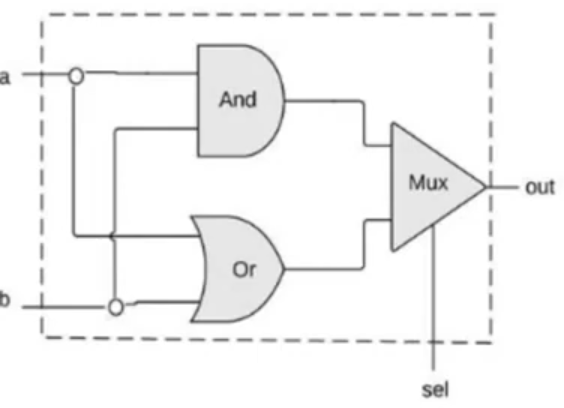
\includegraphics[width=0.4\textwidth]{andMuxOr.png}
\end{figure}

\subsection{Demultiplexor}
\begin{figure}[H]
    \centering
    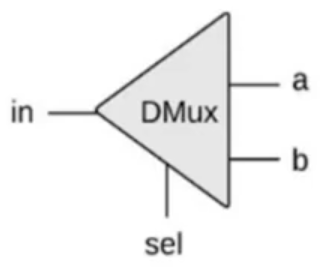
\includegraphics[width=0.4\textwidth]{demux.png}
\end{figure}
$$\text{if sel = 0 then out = a else out = b}$$

\subsection{Bit indexing}
\begin{itemize}
    \item Bit busses are indexed from right to left starting from 0
    \item For example, in a 16-bit bus, the rightmost bit is indexed as 0 and the leftmost bit is indexed as 15
\end{itemize}







%% Continue att 1.7 

\section{Section 2}
%% Continue at 2.1 do this after sections 3 is done
\subsection{Binary representation of numbers}
\begin{itemize}
    \item $1 0 1 0 1 1 = 1 \cdot 2^5 + 0 \cdot 2^4 + 1 \cdot 2^3 + 0 \cdot 2^2 + 1 \cdot 2^1 + 1 \cdot 2^0 = 43$
    \item The value of a binary number is the sum of the values of the bits that are set to 1 
\end{itemize} 

\subsection{Binary addition}
\begin{itemize}
    \item Use addtion with carry over method
    \item For example add $0 0 0 1 0 1 0 1$ and $ 0 1 0 1 1 1 0 0$:
\end{itemize}
\begin{figure}[H]
    \centering
    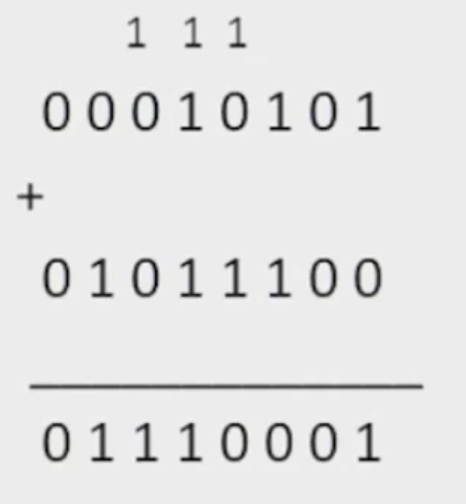
\includegraphics[width=0.25\textwidth]{binaryAddition.png}
\end{figure}

\subsubsection{Overflow}
\begin{itemize}
    \item We cannot go beyond the maximum value that can be represented
    \item This is known as overflow
    \item We will simply ignore the carry bit that goes beyond the maximum value
\end{itemize}

\subsubsection{3 types of Adders}
\begin{itemize}
    \item Half adder --- adds two bits 
    \item Full adder --- adds three bits
    \item Adder --- Adds two 16-bit numbers
\end{itemize}

\subsection{Negative numbers}
2's complement representation:
\begin{itemize}
    \item The number $-x$ is represented as $2^n - x$ where n is the number of bits
    \item All possible positive numbers will be $0 \hdots 2^{n-1} - 1$ 
    \item All possible negative numbers will be $-1 \hdots -2^{n-1}$
    \item This implementation will work for our Adder circuit without any modification 
\end{itemize}

\subsubsection{Negating a number}
\[
-x = 2^n - x = (2^n - 1) - x + 1
\]
\[
2^n - 1 = 111\hdots 11
\]

Example negating $4$ in 8 bits:
\begin{enumerate}
    \item input = $0100$
    \item $1111 - 0100$ = $1011$
    \item $1011 + 1$ = $1100$
    \item $-4$ is represented as $1100$ in 8 bits
    \item output = $1100$
\end{enumerate}

\subsection{ALU -- Arithmetic Logic Unit}
\begin{figure}[H]
    \centering
    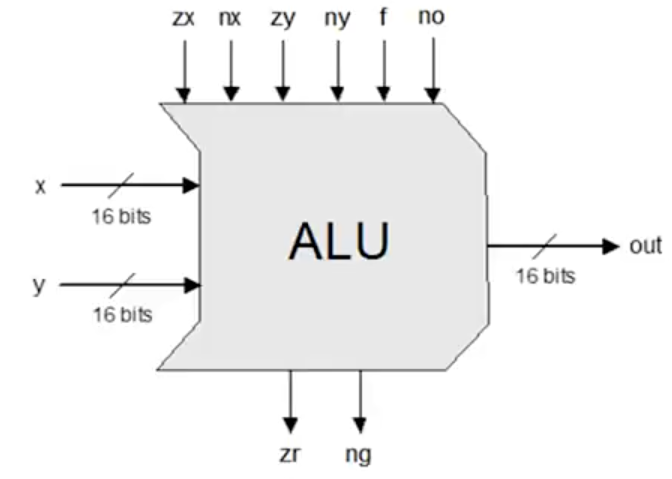
\includegraphics[width=0.5\textwidth]{alu.png}
\end{figure}
\begin{itemize}
    \item ALU computes logical and arithmetic operations
    \item ALU has two 16-bit inputs and one 16-bit output
    \item The ALU can be generalized as $f(in[0], in[1]) = out$ or $f(x, y) = z$
\end{itemize}

\section{Section 3}
\subsection{Sequential logic}
\begin{itemize}
    \item We see time as discrete steps
    \item Computers does not compute everything instantaneously rather stablizes after some time
    \item We choose a clock cycle so that the signal stabilizes 
\end{itemize}

\subsection{Combintorial vs Sequential Logic}
\begin{itemize}
    \item Combinatorial: $out[t] = function(in[t])$
    \item Sequential: $out[t] = function(in[t-1])$
\end{itemize}

\subsection{Flip flops}
\begin{itemize}
    \item In order to move information from $[t-1]$ to $[t]$, we need a storage element called flip flop
    \item DFF (Data Flip Flop) has the functionality: $out[t] = in[t-1]$
    \item At any time unit it returns the output for the previous time unit
    \item The DFF gate is given and not built as a part of the course 
\end{itemize}

\subsection{1-bit Register}
\begin{itemize}
    \item The 1-bit register can remember a single bit of information forever
    \item If load(t-1) then out(t) = in(t-1) else out(t) = out(t-1)
\end{itemize}
\begin{figure}[H]
    \centering
    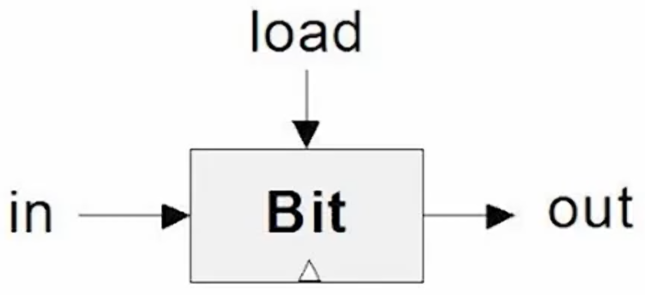
\includegraphics[width=0.65\textwidth]{register.png}
\end{figure}

\subsection{1-bit Register implementation}
\begin{figure}[H]
    \centering
    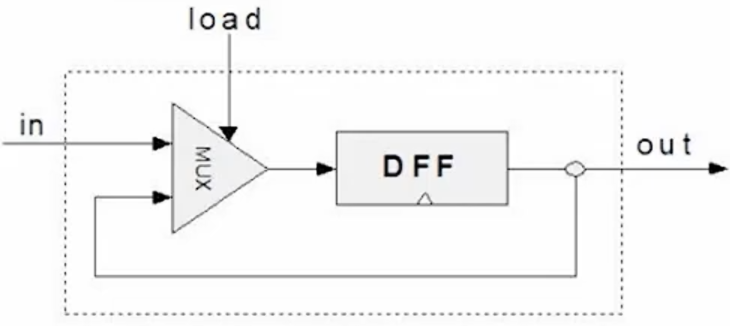
\includegraphics[width=0.75\textwidth]{registerImpl.png}
\end{figure}

\subsection{Memory units: Von Neumann architecture}
\begin{figure}[H]
    \centering
    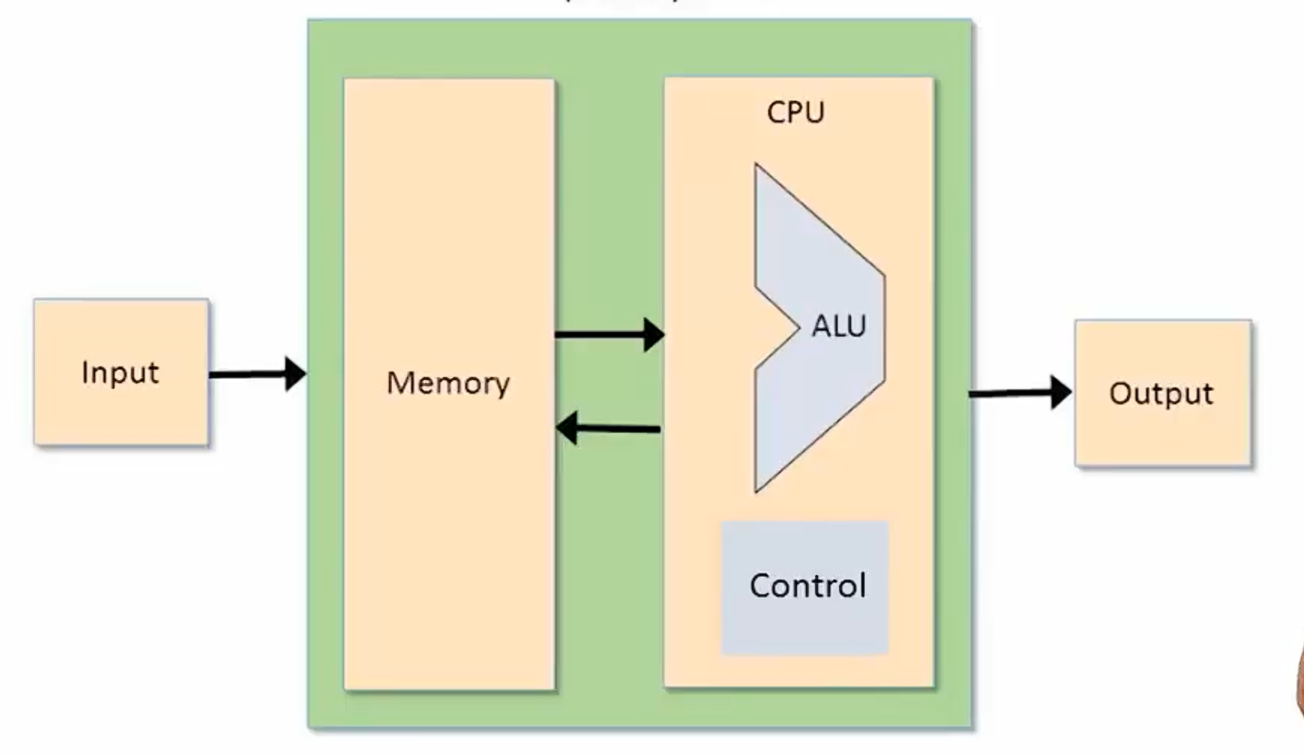
\includegraphics[width=0.75\textwidth]{vonNeumann.png}
\end{figure}

\begin{itemize}
    \item Main memory: RAM (Random Access Memory)
    \item Secondary memory: Disk, memory sticks, etc
    \item Volatile and non-volatile memory
    \item RAM is used for Data and Instructions
\end{itemize}

\subsection{Register: The elemantary building block}
\begin{itemize}
    \item Register has a word width of 16-bits in this course
    \item A register's state is the value that is stored in the register
    \item A 16-bit register consists of multiple 1-bit registers with a load signal
\end{itemize}

\begin{figure}[H]
    \centering
    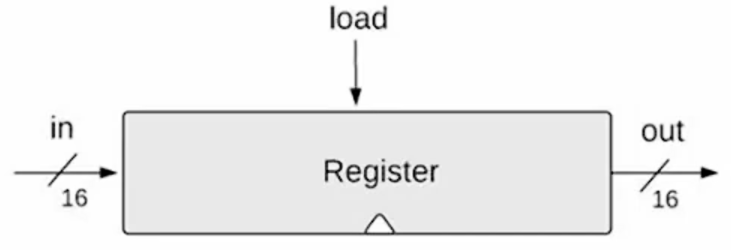
\includegraphics[width=0.75\textwidth]{register16.png}
\end{figure}

\subsection{Write logic}
Suppose we want ot write value $v$ to the register
\begin{itemize}
    \item set $in = v$
    \item set $load = 1$
    \item The register will store and output the value $v$ at the next time unit
\end{itemize}

\subsection{RAM unit}
\begin{figure}[H]
    \centering
    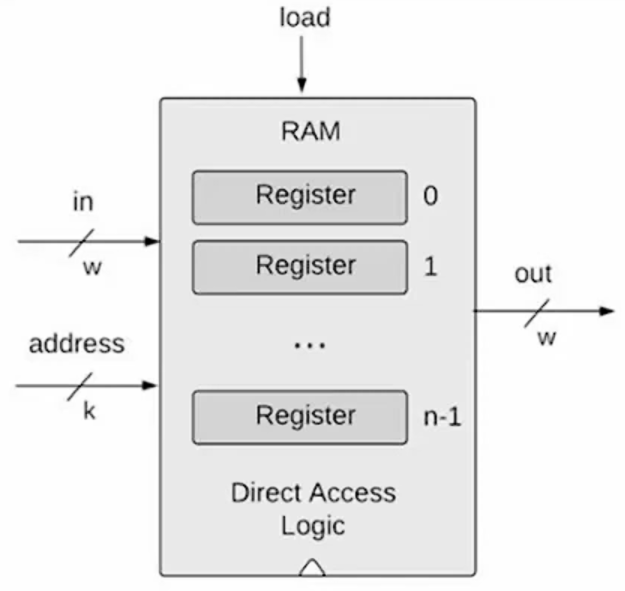
\includegraphics[width=0.75\textwidth]{ram.png}
\end{figure}
\begin{itemize}
    \item RAM unit is a collection of registers 
    \item We can only select one register at a time to read of write
    \item The address is used to select which register 
    \item Given a RAM unit with $n$ registers, we need $\log_2(n)$ bits to map every register
    \item The RAM unit has a load signal, if load = 1 RAM out be writable
\end{itemize}

\subsection{RAM: Read and Write logic}
To read:
\begin{enumerate}
    \item set $address = i$
    \item out: outputs the state of register $i$
\end{enumerate}

To write:
\begin{enumerate}
    \item set $address = i$
    \item set $in = v$
    \item set $load = 1$
    \item The RAM will store the value $v$ 
    \item In the next clock cycle and onwards RAM will write the value $v$
\end{enumerate}

\subsection{The RAM chips we will build}
\begin{figure}[H]
    \centering
    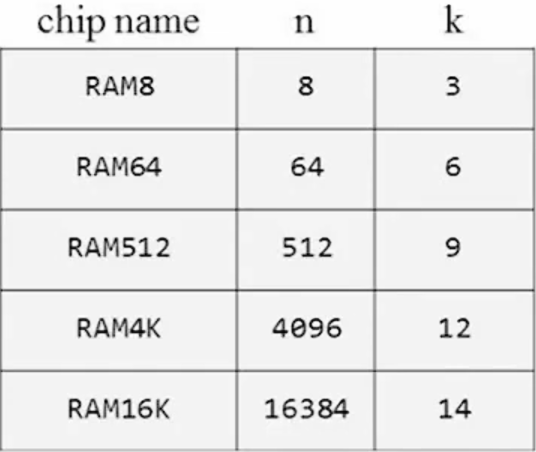
\includegraphics[width=0.3\textwidth]{ramChips.png}
\end{figure}
Regardless of the size of the RAM chip or which register you select every register can be read/written at with the same delay

\subsection{Counters}
Three possible control settings for a counter:
\begin{itemize}
    \item Rest -- $PC = 0$
    \item Next -- $PC++$
    \item Fetch -- $PC = n$
\end{itemize}

\subsection{Counter abstraction}
\begin{figure}[H]
    \centering
    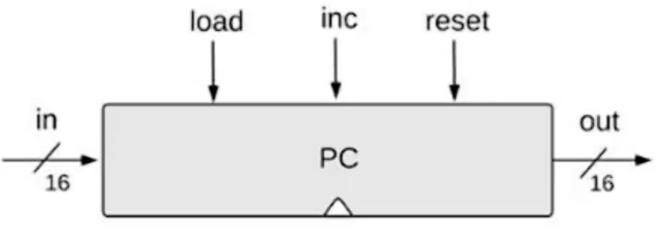
\includegraphics[width=0.75\textwidth]{counter.png}
\end{figure}
\newpage
\subsection{Counter logic}
\begin{itemize}
    \item if (reset == 1) out[t + 1] = 0 -- Resetting the counter
    \item else if (load[t] == 1) out[t + 1] = in[t] -- Setting counter = value
    \item else if (inc[t] == 1) out[t + 1] = out[t] + 1 -- Incrementing the counter
    \item else out[t + 1] = out[t] -- Keep the same value
\end{itemize}

\section{Unit 4} 
\begin{itemize}
    \item Compilation: translating a high-level language into machine language
    \item Instructions like this in the course: $\underbrace{| 0 1 0 0 0 1 0 |}_{\text{ADD}}\underbrace{| 0 0 1 1 |}_{\text{R3}}\underbrace{| 0 0 1 0 |}_{\text{R2}}$
    \item In assembly language it looks like ADD 1, Mem[129]
    \item In assembly we can assume memory location be using index instead of Mem[129] and write ADD 1, index
\end{itemize}

\subsection{Machine Languages: Elements}
There are mainly three different operations:
\begin{itemize}
    \item Arithmetic and logical operations: ADD, SUB, NEG, EQ, GT
    \item Logical operations: AND, OR, NOT
    \item Flow control operations: JMP, JGT, JLT, JEQ
\end{itemize}

\subsection{Registers}
The CPUs usually contains a few registers that are easily accessed

\subsection{Example of different Addressing modes}
\begin{itemize}
    \item Add R1, R2: $R2 \leftarrow R1 + R2$
    \item Add R1, M[200]: Mem[200] $\leftarrow$ R1 + Mem[200]
    \item Add R1, @A: Mem[A] $\leftarrow$ R1 + Mem[A]
    \item Add 73, R1: R1 $\leftarrow$ 73 + R1
\end{itemize}

\subsection{Flow control}
\begin{itemize}
    \item JMP: Unconditional jump to a specific address
    \item JGT: Jump if greater than zero
    \item JLT: Jump if less than zero
    \item JEQ: Jump if equal to zero
\end{itemize}

\subsection{Hack computer: hardware}
\begin{itemize}
    \item Data memory: RAM[0], RAM[1], ..., RAM[16383]
    \item Instruction memory: ROM[0], ROM[1], ..., ROM[32767]
    \item Buses move data between the different components
\end{itemize}

\noindent The hack machine language has two types of instructions:
\begin{itemize}
    \item A-instruction: @value -- value can be a number or a symbol
    \item C-instruction: dest=comp;jump
\end{itemize}

\subsection{Registers}
The hack computer has three registers:
\begin{itemize}
    \item D register: holds a 16-bit value
    \item A register: holds a 16-bit value
    \item M register is the selected RAM location, M = RAM[A]
\end{itemize}

\subsection{A instruction}
\begin{itemize}
    \item A instruction @value
\end{itemize}

Example: @21 means A = 21, M = RAM[21]
\begin{enumerate}
    \item Sets the A register to 21
    \item RAM[21] is selected as the M register
\end{enumerate}

Example set RAM[100] = -1:
\begin{enumerate}
    \item @100
    \item M = -1   
\end{enumerate}

\subsection{C-instruction}
dest = comp; jump
\newline 
The different computations are (comp):
\begin{figure}[H]
    \centering
    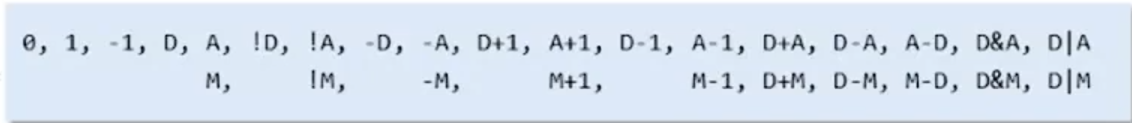
\includegraphics[width=0.75\textwidth]{comp.png}
\end{figure}

\noindent dest can be: null, M, D, MD, A, AM, AD, AMD
jump can be: null, JGT, JEQ, JGE, JLT, JNE, JLE, JMP

\begin{itemize}
    \item Example (if D - 1 == 0 jump to execute the instruction stored in ROM[56])
    \item @56
    \item D - 1; JEQ 
\end{itemize}

\subsection{Hack language specification}
Hack machine language:
\begin{itemize}
    \item A-instructions
    \item C-instructions
\end{itemize}
Hack program = Sequence of instructions written in the Hack machine language 

\subsection{C-instruction}
\begin{itemize}
    \item Symbolic syntax: dest = comp; jump
    \item Binary syntax: $\text{1 1 1 }\underbrace{\text{a c1 c2 c3 c4 c5 c6}}_{\text{comp bits}} \text{ | } \underbrace{\text{d1 d2 d3}}_{\text{dest bits}} \text{ | } \underbrace{\text{j1 j2 j3}}_{\text{jump bits}}$
\end{itemize}

\subsection{I/O devices}
the hack computer has two I/O devices:
\begin{itemize}
    \item Screen: 512 x 256 pixels, each pixel can be black or white
    \item Keyboard: 16-bit code of the key being pressed, 0 if no key is being pressed
\end{itemize}

\subsection{Screen memory map}
\begin{itemize}
    \item The screen is mapped to RAM[16384] to RAM[24575]
    \item Each RAM location corresponds to a 16-pixel row on the screen
    \item Black is represented by 1 and white is represented by 0
    \item Each row is represented by 32 rams (16 pixels per RAM) 16*32 = 512 pixels per row
    \item There are 256 rows, each row is represented by 32 rams, so total 32*256 = 8192 rams for the screen
\end{itemize}

Settings pixel (x, y) to black:
\begin{enumerate}
    \item $i = 32 \cdot row + \frac{col}{16}$
    \item word = Screen[$32 \cdot row + \frac{col}{16}$]
    \begin{itemize}
        \item word = RAM[$16384 + 32 \cdot row + \frac{col}{16}$]
    \end{itemize}
    \item Set the (col mod 16)th bit of word to 1
    \item Commit word to the RAM
\end{enumerate}

\subsection{Keyboard}
The keyboard is mapped to RAM[24576] 
\begin{itemize}
    \item Each key is represented by a unique 16-bit code
    \item If no key is being pressed, RAM[24576] = 0
\end{itemize}

\subsection{Hack programming language part 1}
\subsubsection{A--instructions}
\begin{itemize}
    \item Syntax: @value
    \item value can be a number or a symbol
    \item If value is a number, the A register is set to that number
    \item If value is a symbol, the assembler will translate it to a number and set the A register to that number
\end{itemize}

\subsubsection{C--instructions}
\begin{itemize}
    \item Syntax: dest = comp; jump
    \item dest can be: null, M, D, MD, A, AM, AD, AMD
    \item comp can be: 0, 1, -1, D, A, M, !D, !A, !M, -D, -A, -M, D+1, A+1, M+1, D-1, A-1, M-1, D+A, D+M, D-A, D-M, A-D, M-D
    \item jump can be: null, JGT, JEQ, JGE, JLT, JNE, JLE, JMP
\end{itemize}

\subsubsection{Hack assembler}
\begin{itemize}
    \item Compiles Hack assembly language into Hack machine language
    \item Translates symbolic A-instructions into binary A-instructions
    \item Translates C-instructions into binary C-instructions
\end{itemize}

\subsubsection{Working with registers and memory}
\begin{itemize}
    \item D: Data register 
    \item A: Address register
    \item M: Currently selected RAM location, M = RAM[A]
\end{itemize}

\noindent Example set RAM[10] = 10:
\begin{enumerate}
    \item @10
    \item D = A
\end{enumerate}
Example set D = RAM[17]:
\begin{enumerate}
    \item @17
    \item D = M
\end{enumerate}

\subsubsection{Hack program example: Adding two numbers}
RAM[2] = RAM[0] + RAM[1]
\begin{enumerate}
    \item @0
    \item D = M
    \item @1
    \item D = D + M
    \item @2
    \item M = D
\end{enumerate}

\subsubsection{Terminating a program}
\begin{itemize}
    \item End the program by an infinite loop
    \item For example:
    \begin{enumerate}
        \item @6
        \item 0;JMP 
    \end{enumerate}
\end{itemize}

\subsubsection{Built in symbols}
\begin{itemize}
    \item R0, R1, ..., R15 -- RAM[0] to RAM[15]
    \item Instead of writing @0, we can write @R0, instead of writing @1, we can write @R1, etc
    \item Keep in mind that $R5 \neq r5$ -- Hack is case sensitive
    \item SCREEN -- RAM[16384]
    \item KBD -- RAM[24576]
    \item SP -- RAM[0]
    \item LCL -- RAM[1]
    \item ARG -- RAM[2]
    \item THIS -- RAM[3]
    \item THAT -- RAM[4]
\end{itemize}

\subsection{Hackprogramming part 3}
\subsubsection{Branching}
\begin{itemize}
    \item Branching is used to implement flow control in a program
    \item In Hack we only have goto instructions
\end{itemize}
Example: if R0 > 0 R1 = 1 else R1 = 0
\begin{enumerate}
    \item @R0
    \item D=M
    \item @8
    \item D;JGT
    \item @R1
    \item M=0
    \item @10
    \item 0;JMP
    \item @R1
    \item M=1
    \item @10
    \item 0;JMP
\end{enumerate}

\subsubsection{Labels}
Labels are symbolic references to instruction addresses
\begin{enumerate}
    \item @R0
    \item D=M
    \item @IfPositive
    \item D;JGT
    \item @R1
    \item M=0
    \item @End
    \item 0;JMP
    \item (IfPositive)
    \item @R1
    \item M=1
    \item (End)
    \item @End
    \item 0;JMP
\end{enumerate}
Instead of saying at line 8 we can say at (IfPositive)

\subsubsection{Variabel usage}
for example flipping RAM[0] and RAM[1] using a temp variabel:
\begin{enumerate}
    \item @R1
    \item D=M
    \item @temp
    \item M=D
    \item @R0
    \item D=M
    \item @R1
    \item M=D
    \item @temp
    \item D=M
    \item @R0
    \item M=D
    \item (END)
    \item @END
    \item 0;JMP   
\end{enumerate}
\begin{itemize}
    \item Variables are stoed RAM[16] and onwards
    \item The assembler will automatically allocate memory for variables
\end{itemize}

\subsubsection{Iteration}
Example: Set RAM[0] = 1 + 2 + ... + n
\begin{verbatim}
D=M
@n 
M=D
@i
M=1
@sum
M=0
(LOOP)
@i
D=M
@n
D=D-M
@STOP
D;JGT
@i
D=M
@sum
M=D+M
@i
M=M+1
@LOOP
0;JMP
(STOP)
@sum
D=M
@R1
M=D
(END)
@END
0;JMP    
\end{verbatim}

\subsubsection{Pointers}
For example:
\begin{verbatim}
    for (i = 0, i < n, i++) {
        arr[i] = -i
    }
\end{verbatim}
Would be translated to:
\begin{verbatim}
    // arr = 100
    @100
    D=A
    @arr
    M=D
    // n = 10
    @10
    D=A
    @n
    M=D
    // initialize i = 0
    (LOOP)
    // if (i == n) goto END
    @i
    D=M
    @n
    D=D-M
    @END
    D;JEQ

    // RAM[arr + i] = -1
    @arr
    D=M
    @i
    A=D+M
    M=-1
    // i++
    @i
    M=M+1
    // goto LOOP
    @LOOP
    0;JMP 
    (END)
    @END
    0;JMP
\end{verbatim}

\subsubsection{I/O handling}
\begin{itemize}
    \item Datamemory 0 -- 16384 is for general purpose use
    \item Screen memory is mapped to RAM[16384] to RAM[24575]
    \item Keyboard memory is mapped to RAM[24576]
    \item Screen and keyboard have symbols @SCREEN and @KBD respectively
\end{itemize}

\subsubsection{Pseudo code: rectangle drawing}
\begin{verbatim}
    for (i = 0; i < n; i++) {
        draw 10 black pixels at the beginning of row i
    }
    addr= SCREEN
    n = RAM[0]
    i = 0
    LOOP:
        if (i == n) goto END
        RAM[addr] = 1111111111111111 = -1
        addr = addr + 32
        i = i + 1
        goto LOOP
    END:
        goto END
\end{verbatim}

\subsubsection{Keyboard}
\begin{itemize}
    \item Each key is represented by a unique 16-bit code
    \item If no key is being pressed, RAM[24576] = 0
    \item To read the keyboard, we can simply read the value of RAM[@KBD]
\end{itemize}

\section{Section 5}
\subsection{Von neumann architecture}
\begin{figure}[H]
    \centering
    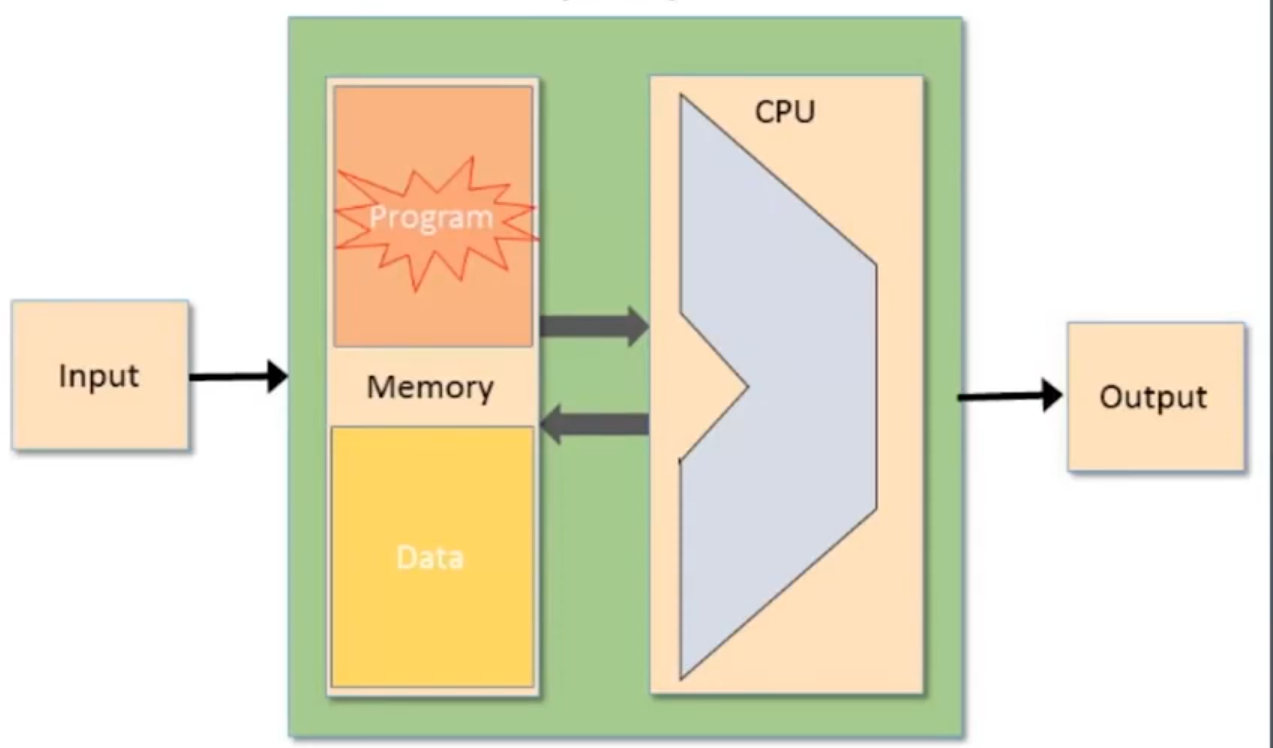
\includegraphics[width=0.75\textwidth]{vonNeumann2.png}
\end{figure}
\begin{itemize}
    \item The CPU has an ALU and registers
    \item The memory has program and data
\end{itemize}

\subsection{Information Flows}
\begin{figure}[H]
    \centering
    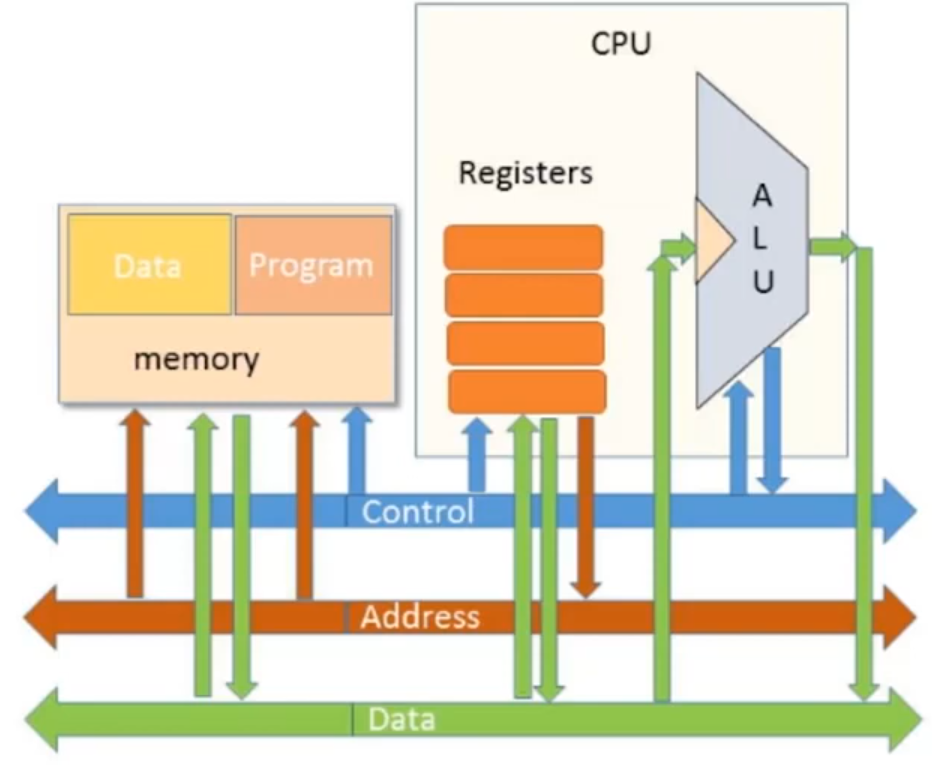
\includegraphics[width=0.75\textwidth]{infoFlow.png}
\end{figure}
\begin{itemize}
    \item Control, Address, Data will be different buses that connects the different components together
\end{itemize}

\subsection{Fetch-Execute Cycle}
The CPU only does two things:
\begin{enumerate}
    \item \textbf{Fetch} instruction from memory
    \item \textbf{Execute} the instruction
\end{enumerate}
The program counter (PC) is used to keep track of which instruction to execute next

\subsubsection{Hierachy of chips parts}
\begin{figure}[H]
    \centering
    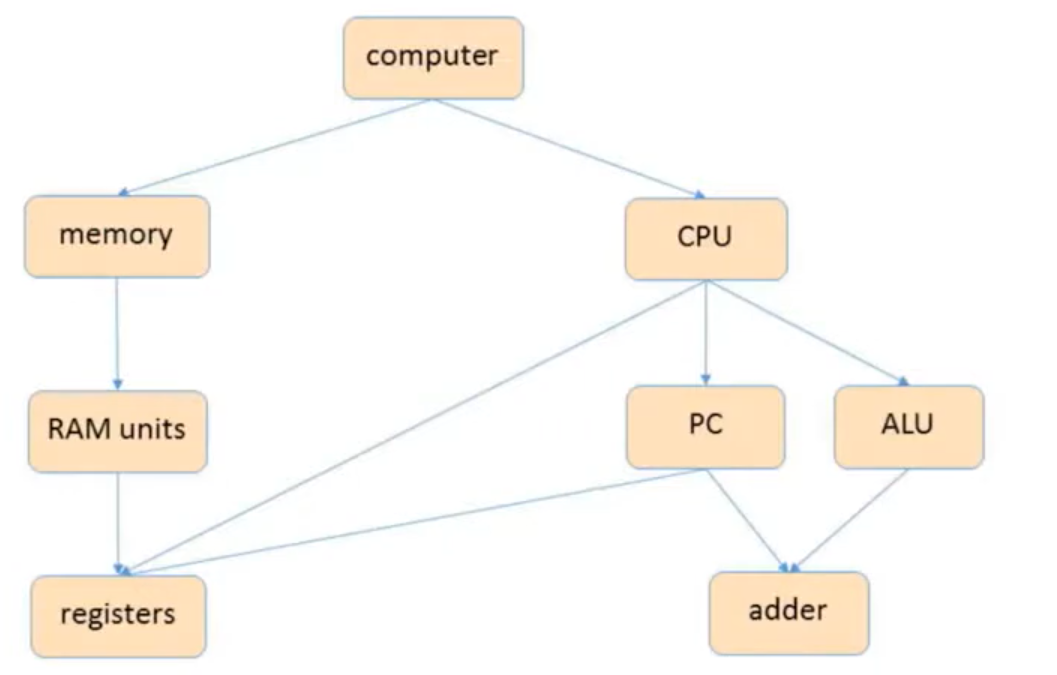
\includegraphics[width=0.65\textwidth]{hierarchy.png}
\end{figure}

\subsubsection{CPU implementation}
\begin{figure}[H]
    \centering
    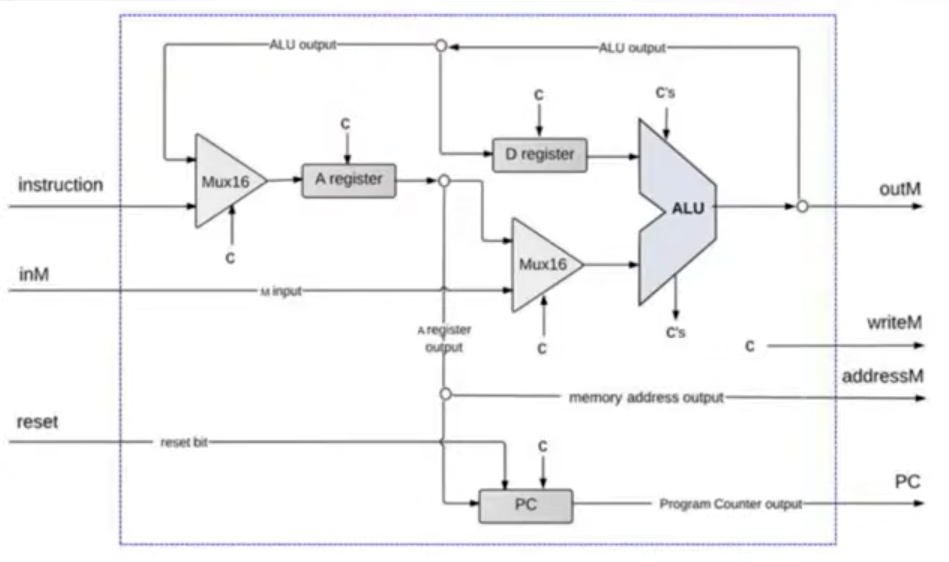
\includegraphics[width=0.85\textwidth]{cpu.png}
\end{figure} 

\subsubsection{Memory abstraction}
\begin{itemize}
    \item \textbf{Address 0 -- 16383:} Data memory
    \item \textbf{Address 16384 -- 24575:} Screen memory
    \item \textbf{Address 24576:} Keyboard memory
\end{itemize}

\subsubsection{ROM implementation}
Basically a RAM with a fixed value that cannot be changed

\subsubsection{Hack computer overview}
\begin{figure}[H]
    \centering
    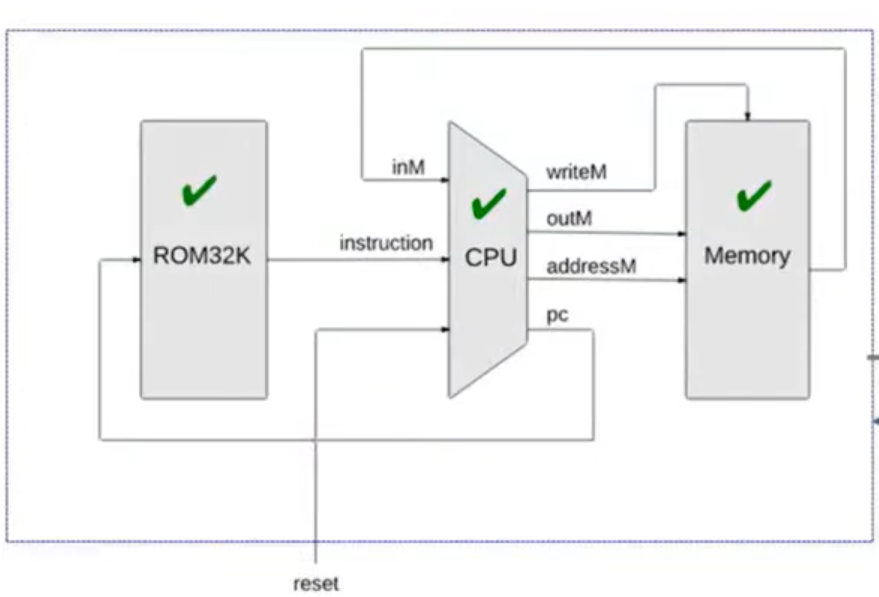
\includegraphics[width=0.75\textwidth]{hackOverview.png}
\end{figure}

\section{Section 6}
\subsubsection{Assembler}
Translates Hack assembly language into Hack machine language by:
\begin{itemize}
    \item Reads next assembly language command
    \item Break it into different field it is composed of
    \item Lookop the binary code for each field
    \item Combine the binary codes into a 16-bit instruction
    \item Output the machine language command 
\end{itemize}

\subsubsection{Symbol handling}
\begin{itemize}
    \item Labels -- i.e JMP, (LOOP), etc
    \item Variables -- i.e temp, i, sum, etc
    \item We need to make map variables to an address
    \item We also need to have a pointer for labels
\end{itemize}

\subsubsection{Forward referecing}
\begin{itemize}
    \item Sometimes we need to jump to a label that we haven't seen yet
    \item Therefore we need two passes of the assembler:
    \begin{enumerate}
        \item First pass: scan the assembly code and record the address of each label
        \item Second pass: translate the assembly code into machine code, using the label addresses recorded in the first pass
    \end{enumerate} 
\end{itemize}

\subsection{The Assembly Process: Handling instructions}
Whitespaces and comments are always ignored by the assembler
\subsubsection{Translating A-instructions}
\begin{itemize}
    \item Symbolic syntax: @value
    \item Which is actually @21
    \item Would be translated to 0000000000010101 in binary
\end{itemize}

\subsubsection{Translating C-instructions}
The C-instruction is always: $\underbrace{\text{dest}}_{\text{Optional}}$ = comp; $\underbrace{\text{jump}}_{\text{Optional}}$ 
which is mapped with table

\subsubsection{Translating symbols}
The symbols are:
\begin{itemize}
    \item R0, R1, ..., R15 -- RAM[0] to RAM[15]
    \item SCREEN -- RAM[16384]
    \item KBD -- RAM[24576]
    \item SP -- RAM[0] (Stack Pointer)
    \item LCL -- RAM[1] (Local segment base address)
    \item ARG -- RAM[2] (Argument segment base address)
    \item THIS -- RAM[3] (This segment base address)
    \item THAT -- RAM[4] (That segment base address)
\end{itemize}
\begin{itemize}
    \item Labels -- (LOOP), (END), etc
    \item Variables -- temp, i, sum, etc
\end{itemize}

\subsection{Handling instructions}
\subsubsection{Translating A--instruction}
\begin{itemize}
    \item @value, eg @21
    \item Translate to binary, eg 0000000000010101
\end{itemize}

\subsubsection{Translating C--instructions}
Generalised to: $\underbrace{\text{dest}}_{\text{Optional}}$=comp; $\underbrace{\text{jump}}_{\text{Optional}}$
\begin{itemize}
    \item Use the comp, dest and jump table to translate the instruction
\end{itemize}

\subsection{Handling symbols}
There are three types of symbols:
\begin{enumerate}
    \item \textbf{Variable symbols:} temp, i, sum, (Represents the locations where the programmer stored values)
    \item \textbf{Label symbols:} (LOOP), (END), etc (Represents the destinations of goto instructions)
    \item \textbf{Predefined symbols:} R0, R1, ..., R15, SCREEN, KBD, SP, LCL, ARG, THIS, THAT (Special memory locations)
    \item The symbols will be mapped to a memory address by the assembler
\end{enumerate}

\subsubsection{Predefined symbols}
\begin{itemize}
    \item There are 23 predefined symbols:
    \item These symbols only appear in A-instructions
\end{itemize}

\subsubsection{Label symbols}
\begin{itemize}
    \item Change the program counter (PC) to the address of the instruction following the label declaration
    \item For example, if we have the instruction (LOOP) at line 10, then the assembler will set the address of LOOP to 10
    \item The assembler will keep track of the address of each label in a symbol table
\end{itemize}

\subsubsection{Variable symbols}
\begin{itemize}
    \item These symbols are represented by an memory address starting with 16
    \item So the first variable symbol will be stored at RAM[16], the second variable symbol will be stored at RAM[17], and so on
    \item A symbol that does not appear as a label will be treated as a variable
\end{itemize}

\subsubsection{Assembly process}
Initialization:
\begin{itemize}
    \item Construct an empty symbol table
    \item Add the pre-defined symbols to the symbol table
\end{itemize}

\noindent First pass:
\begin{itemize}
    \item Scan the entire program 
    \item For each "instruction" of the form (xxx)
    \item Add the pair (xxx, address) to the symbol table, where address is the address of the instruction following the label declaration
\end{itemize}

\noindent Second pass:
\begin{itemize}
    \item Scan the entire program again for each instruction
    \item if the instruction is @symbol, look up the symbol in the symbol table
    \item if not in the symbol table it is an variable, add it to the symbol table and assign it the next available memory address
\end{itemize}

\section{Section 7}
\subsection{Part 2: Summary}
\begin{itemize}
    \item Assembler 
    \item Virtual machine
    \item Compiler
    \item Operating system
\end{itemize}
\subsubsection{From high level to low level}
\begin{figure}[H]
    \centering
    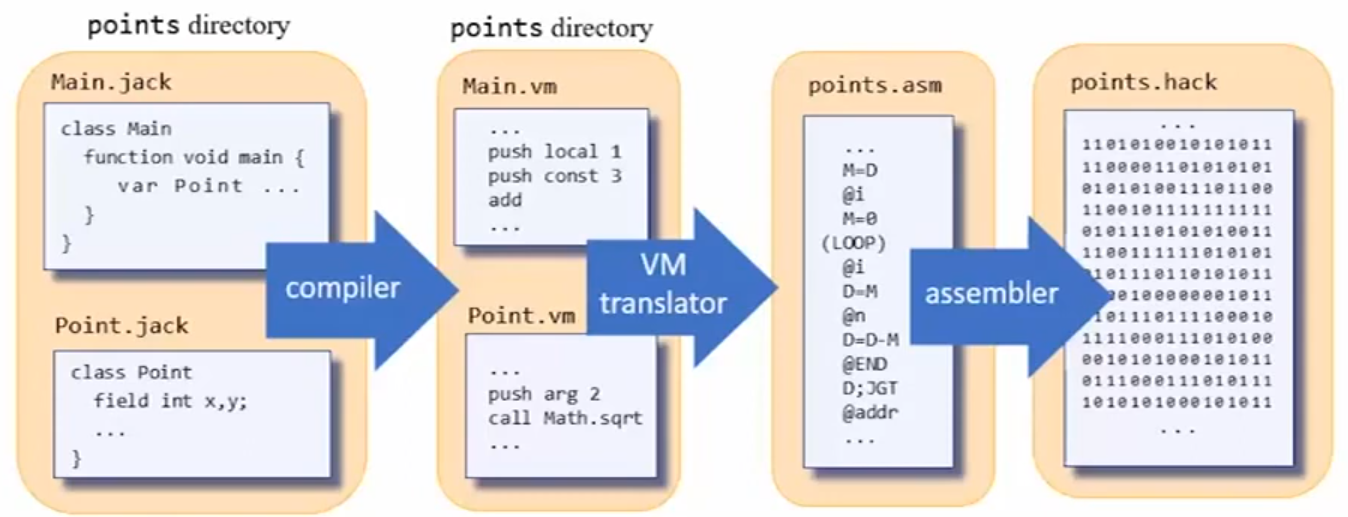
\includegraphics[width=0.75\textwidth]{highToLow.png}
\end{figure}

\subsection{Program Compilation}
Instead of writing a compiler in every language we do like Java "write once run anywhere"
\begin{itemize}
    \item Jack just like Java uses two tier compilation instead of compiling directly to binary
    \item Java comiples to bytecode which is run on the Java Virtual Machine (JVM)
\end{itemize}

\subsection{VM abstraction -- The stack}
\begin{itemize}
    \item The datastructure stack is like a stack of plates
    \item The stack has these operations:
    \begin{itemize}
        \item \textbf{Push:}Adds a plate at the stack's top
        \item \textbf{Pop: }Removes the top plate
        \item \textbf{Add: }Adds the top two plates and pushes the result back on the stack
        \item \textbf{Neg: }Negates the top plate and pushes the result back on the stack 
        \item \textbf{eq: }Check equal for top two plates and pushes 1 if they are equal and 0 if they are not equal
        \item \textbf{or: }Check if either of the top two plates is non-zero and pushes 1 if true and 0 if false
    \end{itemize}
    \item \textbf{Stack pointer (SP):} Points to the next empty slot on the stack
\end{itemize}

\subsection{VM abstraction: Memory segments}
The VM has 8 memory segments:
\begin{enumerate}
    \item local
    \item argument
    \item this 
    \item that 
    \item constant 
    \item static 
    \item pointer 
    \item temp
\end{enumerate}

\subsection{VM implementation: The stack}
\subsubsection{Pointer manipulation}
\begin{itemize}
    \item We store the address of the top of the stack in RAM[0] (@SP)
    \item When we add something to the stack, we write it to RAM[SP] and then increment SP
    \item When we pop something from the stack, we decrement SP and then read the value from RAM[SP]
\end{itemize}

\subsection{VM implementation: Memory segments}
The memory segment pointers are
\begin{itemize}
    \item local segment pointer: RAM[1] (@LCL)
    \item argument segment pointer: RAM[2] (@ARG)
    \item this segment pointer: RAM[3] (@THIS)
    \item that segment pointer: RAM[4] (@THAT)
    \item temp segment pointer: RAM[5] (@TEMP)
    \item THIS stores stores field variables of the current object
    \item THAT stores the array that is currently being manipulated
\end{itemize}

\subsubsection{Local implementation}
\begin{itemize}
    \item We use @LCL to point to the base of the local segment
    \item To access the ith local variable, we can compute the address as LCL + i and then read/write to that address
\end{itemize}

\subsubsection{Constant implementation}
\begin{itemize}
    \item Constant segment does not have a memory location
    \item We push constant by pushing onto the stack the value of the constant and advancing SP
\end{itemize}

\subsubsection{Static implementation}
\begin{itemize}
    \item Stores all static variables of a program  
    \item Static variables are seen by all methods in a program
    \item We do this by staring static variables as assembly variables which will be mapped RAM[16] and onwards
\end{itemize}

\begin{verbatim}
    // pop static 5
    @Foo.5
    M=D

    // pop static 2
    @Foo.2
    M=D
\end{verbatim}
                        
\subsubsection{Temp implementation}
\begin{itemize}
    \item temp is a fixed 8 place memory segment
    \item Mapped to RAM[5] to RAM[12]
\end{itemize}

\subsubsection{Pointer implementation}
\begin{itemize}
    \item The poiner segment is fixed and points to 2 locations
    \item pointer 0 points to THIS (RAM[3])
    \item pointer 1 points to THAT (RAM[4])
    \item push pointer 0 means push the value of THIS onto the stack
    \item push pointer 1 means push the value of THAT onto the stack
    \item pop pointer 0 means pop the top of the stack and store it in THIS
    \item pop pointer 1 means pop the top of the stack and store it in THAT
\end{itemize}

\subsection{VM emulator}
The VM emulator is a program that takes a VM program as input and executes it by simulating the stack and memory segments

\subsection{VM implementation}
\subsubsection{VM translator}
\begin{itemize}
    \item Translates VM code into Hack assembly 
    \item Each VM command gets translated into a sequence of Hack assembly instructions
\end{itemize}

\subsection{Hack ram mapping}
\begin{figure}[H]
    \centering
    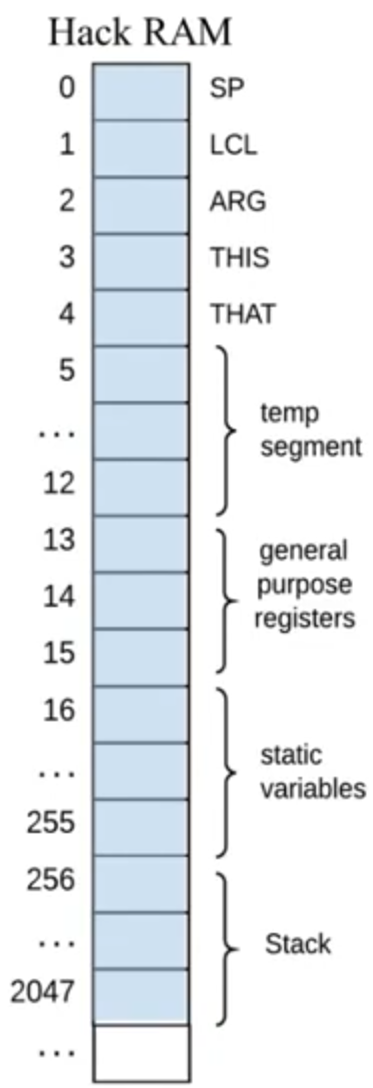
\includegraphics[width=0.25\textwidth]{hackRam.png}
\end{figure}

The standard symbols are:
\begin{itemize}
    \item SP -- RAM[0]
    \item LCL -- RAM[1]
    \item ARG -- RAM[2]
    \item THIS -- RAM[3]
    \item THAT -- RAM[4]
    \item R13-R15 -- RAM[13] to RAM[15]
    \item Xxx.i -- static variable i in file Xxx.asm, mapped to RAM[16] and onwards
\end{itemize}

\subsection{Program flow control}
\begin{itemize}
    \item Abstraction: Using functions to abstract away details
    \item Branching: Control the order of execution of instructions
\end{itemize}
Branching commands in VM:
\begin{itemize}
    \item \textbf{label: }Defines a label that can be used as a goto destination
    \item \textbf{goto: }Unconditional jump to a label
    \item \textbf{if-goto: }Conditional jump to a label if the
    \item the if command evaluates the top of the stack
\end{itemize}

\subsection{Functions}
\begin{itemize}
    \item Caller -- the function that calls another function
    \item Callee -- the function gets called by another function
\end{itemize}
\subsubsection{Calling a function}
Calling a function involves:
\begin{itemize}
    \item Pushing the arguments onto the stack
    \item Calling the function using the call command
\end{itemize}
\begin{verbatim}
push x
push 17
sub
push 5
call Math.multiply 
add
call Math.sqrt
\end{verbatim}

\subsubsection{Defining a function}
Defining a function involves:
\begin{verbatim}
function <name> <nVars>

// function body

return 
\end{verbatim}
\begin{itemize}
    \item The last pushed value before return is the return value
\end{itemize}

\subsection{Function call return}
\subsubsection{Function execution}
\begin{itemize}
    \item During a given point only a few functions are executing 
    \item Calling chain is the chain of functions that are currently executing
\end{itemize}

\subsubsection{Function run-time}
\begin{itemize}
    \item Each function uses a working stack + memory segments
    \item The working stack + memory segments are initiated when the functions runs 
    \item They are recycled when the function returns
\end{itemize}

The function replaces the arguments in the caller stack with the return value
\begin{itemize}
    \item When the function calls nArgs we use the argument pointer to find the arguments
    \item Function sets arg and saves the caller frame
    \item The frame is return address, local, argument, this and that
\end{itemize}

\subsubsection{Return command}
\begin{itemize}
    \item We take the top value of the function stack and copy to argument 0
    \item Restore the segment pointer of the caller
    \item Clears the function stackk
    \item Sets stack pointer for the caller
    \item Jumps to the return address within the caller's code
\end{itemize}

\subsubsection{The global stack}
\begin{itemize}
    \item The global stack is the stack that is used by all functions in a program
    \item Each function has its own working stack which is a portion of the global stack
\end{itemize}
\newpage
\subsection{Function -- Run-time simulation}
Example of recursive function factorial(n):
\begin{verbatim}
int main() {
    return factorial(3);
}
// Returns n!
int factorial(int n) {
    if (n == 1)
        return 1;
    else
        return n * factorial(n - 1);
}
\end{verbatim}
In pseudo code:
\begin{verbatim}
function main
    push 3
    call factorial
    return 

function factorial
    push n 
    push 1
    eq
    if-goto BASECASE
    push n
    push n
    push 1
    sub 
    call factorial
    call mult
    return
\end{verbatim}
In actual VM code:
\begin{verbatim}
function main 0
    push constant 3
    call factorial 1   // 1 is the number of arguments
    return 

functoin factorial 0
    push argument 0
    push constant 1
    eq 
    if goto BASECASE
    push argument 0
    push argument 0 
    push constant 1 
    sub 
    call factorial 1
    call mult 
    return 
\end{verbatim}

\subsubsection{Visualization}
\begin{figure}[H]
    \centering
    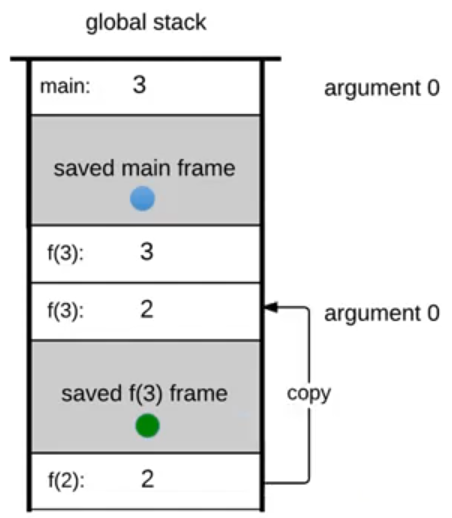
\includegraphics[width=0.3\textwidth]{functionCall.png}
\end{figure}

\subsection{Function implementation}
The callee function process:
\begin{enumerate}
    \item Argument is initialized by the caller
    \item Local segment is initialized to 0
    \item Static segment is shared by all functions
    \item Working stack is empty 
    \item Before returning the push value onto the stack  
\end{enumerate}

\subsubsection{Handling a call}
\textbf{VM command: } call <functionName> <nArgs>
\begin{verbatim}
    push returnAddress  // Where the function should return value
    push LCL  // Save the caller's LCL
    push ARG  // Save the caller's ARG
    push THIS  // Save the caller's THIS
    push THAT  // Save the caller's THAT
    ARG = SP - nArgs - 5  // Reposition ARG for the callee
\end{verbatim}

\subsection{Operating system}
Only the math and memory is in the exam
\subsection{Efficiency matter}
\subsubsection{Multiplication}
Stack the numbers on top of each other and multiply algorithmically
\begin{itemize}
    \item Shift the first number and add if the second number is 1
\end{itemize}
\begin{figure}[H]
    \centering
    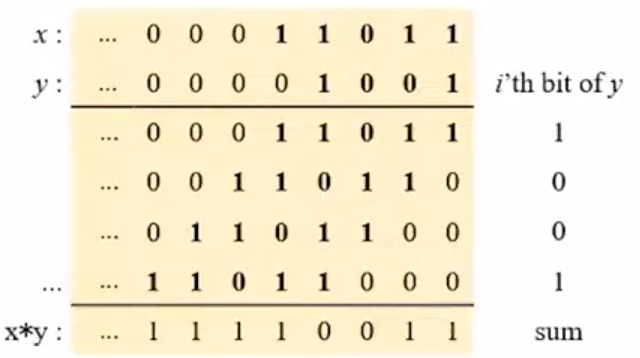
\includegraphics[width=0.75\textwidth]{multi.png}
\end{figure}
Now we can multiply in O(log n) time instead of O(n) time

\newpage
\subsection{Mathematical operations} 
\subsection{Naive division}
\begin{itemize}
    \item Subtract the divisor from the dividend until the remainder is less than the divisor
    \item The algorithm runs in O(n) time 
\end{itemize}

\subsection{Long division algorithm}
By implementing the long division algorithm we can divide in O(log n) times

\subsection{Recursive division algorithm}
\begin{verbatim}
// Same idea as binary search
divide(x, y)
    if (y > x) return 0
    q = divide(x, 2*y)
    if ((x-1 * q * y) < y)
        return 2*q
    else
        return 2*q + 1
\end{verbatim}

\subsection{Square root algorithm}
\begin{verbatim}
sqrt(x)
    y = 0
    for j = n/2 - 1... do
        if (y+2^j)^2 <= x then
            y = y + 2^j
    return y
\end{verbatim}

\subsection{Max/min function}
Trivialt

\subsection{Multiplication algorthm pseudocode}
\begin{verbatim}
multiply(x, y)
    sum = 0
    shiftedX = x
    for i = 0...w-1 do
        if ((i'th bit of y) == 1)
            sum = sum + shiftedX
        shiftedX = shiftedX << 1
    return sum 
\end{verbatim}

\subsection{Negative numbers}
\begin{itemize}
    \item Negative numbers will work and handled just fine
    \item Overflow will be handled the first 16 bit will be correct
    \item Dividing negative numbers we can simply divide absolute values then add a minus sign 
\end{itemize}

\subsection{Bit shifting}
\begin{itemize}
    \item The Jack language does not have bit shifting operations
    \item We can use arrays to implement bit shifting
    \item For example, to shift x to the left by 1 bit, we can simply multiply x by 2
\end{itemize}

\subsection{Memory management}
\begin{itemize}
    \item Peek -- Read a value from a memory location without modifying it
    \item Poke -- Write a value to a memory location
\end{itemize}

\subsection{Heap}
Objects and arrays are allocated on the heap, which is a region of memory that is used for dynamic memory allocation
\begin{itemize}
    \item alloc -- Allocate a block of memory on the heap and return its address
    \item dealloc -- Recycles a block of memory on the heap given its address
\end{itemize}
Assume we create a object then the stack will point to the address of the object on the heap

\subsection{Heap management}
Initialization:
\begin{itemize}
    \item free = heapBase -- The entire heap is free at the beginning
    \item alloc(size):
    \begin{itemize}
        \item Assume we want to allocate a block of memory of size 3
        \item We go from free to free + size and mark those memory locations as allocated
        \item We then update free to free + size
        \item Then return the block to the caller
    \end{itemize}
    \item deAlloc(Object): 
    \begin{itemize}
        \item Keep track of allocated blocks as a linked list
    \end{itemize}
\end{itemize}

\subsection{Segment illustration}
\begin{itemize}
    \item Each segment contains two blocks: a next segment pointer and block size 
    \item When alloc(size) is called we traverse the linked list of segments until we find a free segment with size >= size
    \item When append the dealloced block to the freeList
\end{itemize}

\subsection{alloc(size) function}
When we allocate a block we search the freeList with these algorithm:
\begin{itemize}
    \item First fit: Allocate the first block that is big enough
    \item Best fit: Allocate the smallest block that is big enough
\end{itemize}

\subsection{deAlloc(object) function}
When deallocating a block we simply append the block to the freeList however this will fragment the freeList

\subsection{Defragmentation}
\begin{itemize}
    \item We can defragment the freeList by merging adjacent free blocks into a single block
    \item This will reduce fragmentation and make it easier to find large blocks of memory
\end{itemize}

\subsection{Initiating the heap}
\begin{itemize}
    \item heapBase = 2048
    \item freeList = heapBase
    \item heap[0] = 0 // next segment pointer
    \item heap[1] = 32768 - heapBase // block size
\end{itemize}
After memory has been allocated and deallocated freeList will change
\begin{itemize}
    \item The freeList variable points to the first free block of memory on the heap
    \item Each memory block has the size and points to the next free block of memory
    \item When we allocate a block of memory we update the freeList to point to the next free block of memory
\end{itemize}

\subsection{Lexical analysis}
\begin{figure}[H]
    \centering
    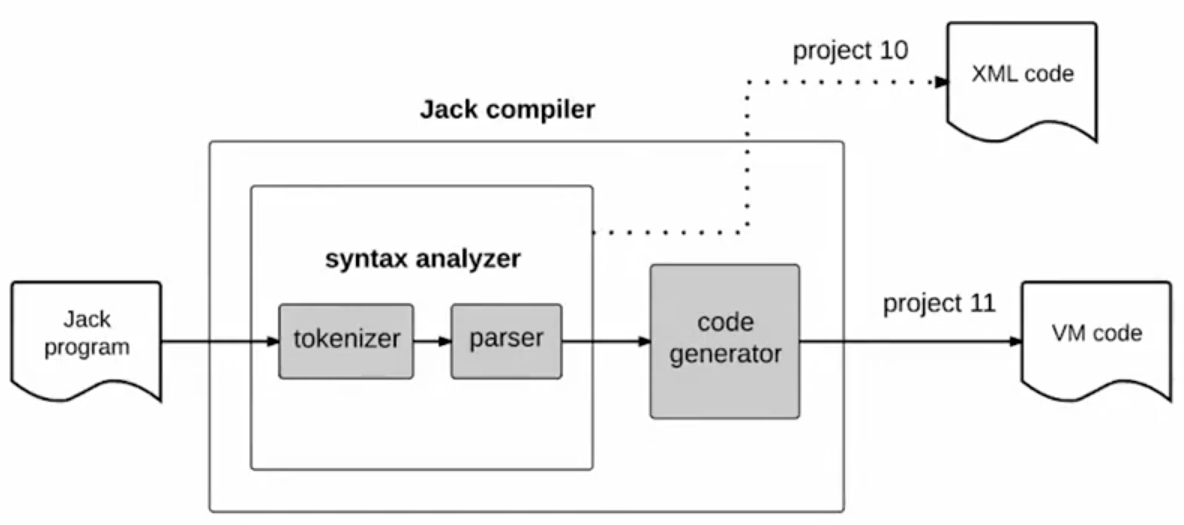
\includegraphics[width=0.7\textwidth]{jackcomp.png}
\end{figure}

\subsection{Tokenizing}
In order to compile we need to tokenize the code first
\begin{figure}[H]
    \centering
    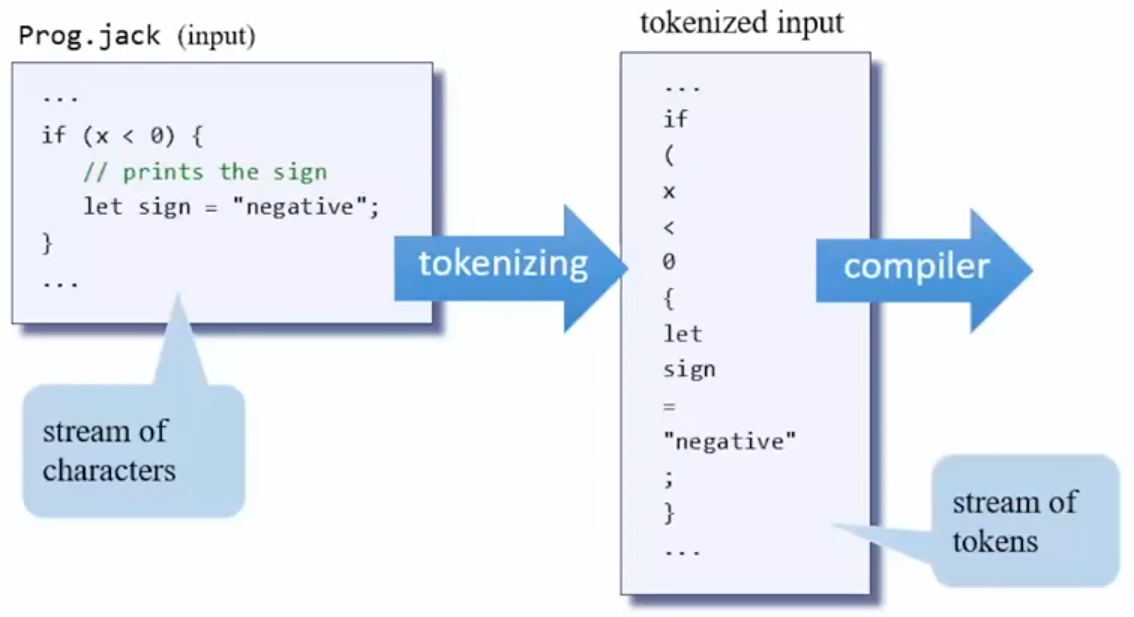
\includegraphics[width=0.75\textwidth]{tokenizing.png}
\end{figure}

\subsubsection{5 category of tokens}
\begin{itemize}
    \item Keyword -- class, constructor, function, method... 
    \item Symbol -- { } ( ) [ ] . , ; + - * / \& | < > = ~
    \item integerConstant -- 0, 1, 2, ..., 32767
    \item StringConstant -- "Here is a string constant not including the double quotes"
    \item Identifier -- to represent variable names, class names, method names, etc can start with a letter or an underscore
\end{itemize}
Tokenizer process:
\begin{enumerate}
    \item The tokenizer reads the input stream and breaks it into tokens
    \item The tokenizer ignores whitespace and comments
    \item The tokenizer surrounds each token with <tokenType> token </tokenType> tags and outputs the result with one token per line
\end{enumerate}

\subsection{Grammar}   
Terminal and non-terminal rules:
\begin{itemize}
    \item Terminal rules: Right hand side consists of constants only
    \item Non-terminal rules: Right hand side contains at least one non-terminal
\end{itemize}

\subsubsection{Jack grammar}
\begin{itemize}
    \item statement: ifStatement | whileStatement | letStatement 
    \item ifStatement: 'if' '(' expression ')' '{' statement* '}' 
    \item The rest is available in the exam handbook
    \item Parsing is determining if a given input conforms to the grammar
\end{itemize}

\subsubsection{Parse tree}
Parse trees can be represented as a tree structure or as an XML file
\begin{figure}[H]
    \centering
    \begin{minipage}[t]{0.42\textwidth}
        \vspace{0pt}
        \centering
        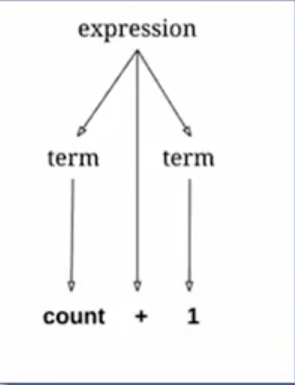
\includegraphics[width=\linewidth]{parsetree.png}
    \end{minipage}\hfill
    \begin{minipage}[t]{0.52\textwidth}
        \vspace{0pt}
        \begin{verbatim}
<expression>
    <term>
        <identifier> count </identifier>
    </term>
    <symbol> + </symbol>
    <term>
        <integerConstant> 1 </integerConstant>
    </term>
</expression>
        \end{verbatim}
    \end{minipage}
\end{figure}

\subsection{Handling variables}
Assume the code is sum = x * (1 + rate);
\begin{itemize}
    \item x is argument 2
    \item rate is static 0
\end{itemize}
The vm code for this would be:
\begin{verbatim}
push argument 2
push constant 1
push static 0 
add 
call Math.multiply 2
pop local 3
\end{verbatim}
Different variable types are stored in different memory segments:
\begin{itemize}
    \item Class level variables
    \begin{itemize}
        \item field 
        \item static
    \end{itemize} 
    \item Subroutine level variables
    \begin{itemize}
        \item argument
        \item local
    \end{itemize}
\end{itemize}
Each variable as 4 properties:
\begin{itemize}
    \item name -- identifer of the variable
    \item type -- int, char, boolean, class type
    \item kind -- field, static, local, argument
    \item scope -- class level, subroutine level
\end{itemize}

\subsubsection{Symbol table}
Always <name, type, kind, scope>
\begin{figure}[H]
    \centering
    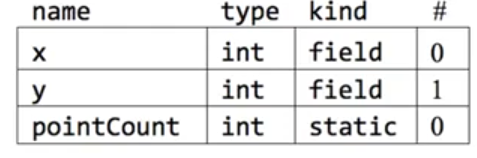
\includegraphics[width=0.75\textwidth]{symbolTable.png}
\end{figure}

Each time we compile we need two symbol tables:
\begin{itemize}
    \item Class level symbol table -- for class level variables
    \item Subroutine level symbol table -- for subroutine level variables
\end{itemize}

\subsubsection{Nested scoping}
In java you can create variables in nested scopes, for example:
\begin{verbatim}
void foo() {
    method bar() {  // scop 1
        // variables declared here are in the scope of bar
        {  // scope 2
            // variables declared here are in the scope of the block within bar
        }
    }
}
\end{verbatim}
We can use a stack of symbol tables to handle nested scoping:
\begin{figure}[H]
    \centering
    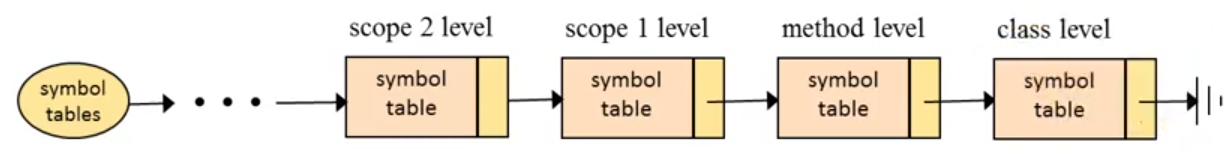
\includegraphics[width=1\textwidth]{nestedScope.png}
\end{figure}

\subsection{Handling expressions}
The stack oriented VM makes expressions post fix while the language is infix so we need to convert infix to post fix:
\begin{verbatim}
    if exp is a number n:
        output "push n"
    
    if exp is a variable var:
        output "push var"
    
    if exp is "exp_1 op exp_2":
        compile exp_1
        compile exp_2
        output "op"
    
    if exp is "op exp":
        compile exp
        output "op"
    
    if exp is "f(exp_1, exp_2, ..., exp_n)":
        compile exp_1
        compile exp_2
        ...
        compile exp_n
        output "call f n"
\end{verbatim}
The jack language does not have operator priority the language features parentheses to specify the order of operations

\subsection{Handling objects}
\begin{itemize}
    \item Object data is accessed through the THIS segment
    \item Array data is accessed through the THAT segment
    \item Local and argument are on the stack
    \item This and that are on the heap
\end{itemize}
\begin{verbatim}
    // set THIS to 8000
    push constant 8000
    pop pointer 0
\end{verbatim}
Example of RAM[8000] = 123 and THIS[0] = 123:
\begin{verbatim}
    push 8000
    pop pointer 0
    push constant 123
    pop this 0
\end{verbatim}

\subsection{Objects construction}
Assume this code:
\begin{verbatim}
    var Point p1, p2;
    var int d;

    let p1 = Point.new(2, 3);
    let p2 = Point.new(5, 7);
\end{verbatim}
The symbol table after the first two lines would be:
\begin{itemize}
    \item <name> <type> <kind> <scope> 
    \item p1 Point local 0
    \item p2 Point local 1
    \item d int local 2
\end{itemize}
The vm code for the last two lines would be:
\begin{verbatim}
    push constant 2
    push constant 3
    call Point.new 
    
    // p1 is the base address of the new object, we want p1 to point to the new object
    pop p1
\end{verbatim}
\begin{itemize}
    \item When declaring variables we only allocate memory of the base address of the object
    \item Only when object is constructed will the variable point to the actual object on the heap
\end{itemize}

\subsubsection{Compiling constructors}
Lets assume we have the following constructor:
\begin{verbatim}
class Point {
    field int x, y;
    static int pointCount;

    constructor Point new(int ax, int ay) {
        let x = ax;
        let y = ay;
        let pointCount = pointCount + 1;
        return this;
    }
}
\end{verbatim}
Focusing on the constructor part:
\begin{verbatim}
// Two argument are passed to the constructor, ax and ay
push 2 
call Memory.alloc 1 
pop pointer 0 // set THIS to point to the new object
// after the constructor runs it return the address of the new object
\end{verbatim}

\subsection{Object manipulation}
Example of object manipulation:
\begin{verbatim}
    var Point p1, p2, p3;
    var int x, d;

    let p1 = Point.new(2, 3);
    let p2 = Point.new(5, 7);

    let x = p1.x;    
    let p3 = p1.plus(p2);
    let d = p1.distance(p2);
\end{verbatim}
\begin{enumerate}
    \item Push the object pointer onto the stack
    \item Push the arguments on the stack
    \item call the method
\end{enumerate}

Example of compiling a class method call:
\begin{verbatim}
    // let d = p1.distance(p2); becomes

    push argument 0 // Currently operating object is argument 0 
    pop pointer 0 // set THIS to the currently operating object
    // let dx = x - other.getx();
    push this 0 
    push argument 1
    call Point.getx 1
    sub 
    pop local 0 // dx is local 0
\end{verbatim}

Compling void method that does not return a value:
\begin{itemize}
    \item The method will manipulate the symbol table
    \item We will simply return 0, which is a dummy value
    \item Then we pop temp 0 to discard the dummy return value
\end{itemize}

\subsection{Handling Arrays}
Array declaration:
\begin{itemize}
    \item When we declare an array be \textit{var Array arr;} we put local 0 to 0
    \item When we construct an array by \textit{let arr = Array.new(10);} we allocated a block of 10 memory on the heap and set local 0 to point to the base address of the array
    \item var Array arr; does not generate code only changing to symbol table
\end{itemize}

Array manipulation:
\begin{itemize}
    \item Use THIS to represent the values of the current object
    \item Use THAT to represent the values of the current array
\end{itemize}

Supposed that we want to RAM[8056] = 17
\begin{verbatim}
    push constant 8056
    pop pointer 1 
    push constant 17
    pop that 0
\end{verbatim}

Example arr[2] = 17;
\begin{verbatim}
    push arr  // base address of the array
    push constant 2 
    add 
    pop pointer 1
    push constant 17
    pop that 0
\end{verbatim}
Advantage with VM is that the code won't escape the VM RAM therefore it is safer
  
\subsubsection{Generalized array access}
\begin{verbatim}
    // a[i] = b[j]
    push a 
    push i
    add 
    pop pointer 1

    // now handle b[j]
    push b
    push j
    add 
    pop pointer 1 
    push that 0
\end{verbatim}
This code does not work because we overwrite the pointer when handling b[j] instead we should do this:
\begin{verbatim}
    push a 
    push i 
    add
    push b
    push j 
    add
    pop pointer 1
    push that 0 
    pop temp 0  
    pop pointer 1
    push temp 0
    pop that 0 
\end{verbatim}
In summary always use temp to store intermediate values when handling arrays


\newpage
\section*{Tenta analys}
\subsection*{Fråga 1 på tentan}
\subsubsection*{Boolean Algebra \& ALU Logic Proofs}
\textbf{Core concept:} The exams frequently ask you to prove how the ALU computes a specific output (e.g., $out = 1$) or to simplify logic gates (e.g., XOR) using pure Boolean algebra, \textit{not} truth tables.
\begin{itemize}
    \item \textbf{XOR Simplification:} 
    $x \oplus y = (\overline{x} \cdot y) + (x \cdot \overline{y})$. 
    A common exam proof is showing $x \oplus x = 0$:
    $$x \oplus x = (\overline{x} \cdot x) + (x \cdot \overline{x}) = 0 + 0 = 0$$
    \item \textbf{ALU Output Proofs (e.g., computing $out = 1$):}
    The ALU uses 6 control bits: \texttt{zx, nx, zy, ny, f, no}. To output $1$, the control bits are usually all set to $1$. The mathematical proof is:
    \begin{itemize}
        \item \texttt{zx=1, nx=1}: Input $x$ is zeroed ($00\dots0$), then negated ($11\dots1$). In 2's complement, all 1s equals $-1$.
        \item \texttt{zy=1, ny=1}: Input $y$ is similarly zeroed and negated, becoming $-1$.
        \item \texttt{f=1}: The ALU performs addition: $x + y \rightarrow -1 + -1 = -2$. In binary, $-2$ is $11\dots110$.
        \item \texttt{no=1}: The output is bitwise negated. $\text{NOT}(11\dots110) = 00\dots001$, which equals $1$.
    \end{itemize}
\end{itemize}

\subsubsection*{Binary Arithmetic \& 2's Complement}
\textbf{Core concept:} Performing manual subtraction or addition using binary to show how the hardware processes it.
\begin{itemize}
    \item \textbf{Formula for negative numbers:} $-x = \text{NOT}(x) + 1$
    \item \textbf{Example Proof ($4 - 5 = -1$):}
    \begin{itemize}
        \item Represent $4$ in binary (e.g., 4 bits): $0100$
        \item Represent $5$ in binary: $0101$
        \item Convert $5$ to $-5$ using 2's complement: $\text{NOT}(0101) = 1010$. Add $1$: $1010 + 1 = 1011$ (This is $-5$).
        \item Add $4$ and $-5$: $0100 + 1011 = 1111$.
        \item The result $1111$ in 2's complement represents $-1$.
    \end{itemize}
\end{itemize}

\subsubsection*{Combinational vs. Sequential Logic (Chip Design)}
\textbf{Core concept:} Knowing when to use memory (state) vs pure logic, and how to construct mid-level chips using basic parts (Mux, Add16, Not16).
\begin{itemize}
    \item \textbf{Sequential vs Combinational:} A chip is \textit{sequential} if it contains a storage element (like a DFF or Register) to hold a state across clock cycles (e.g., a multiplier that adds repeatedly needs a register to store the running sum). If output depends \textit{only} on current inputs, it is \textit{combinational}.
    \item \textbf{Example Chip Design (Absolute Value / \texttt{Abs16}):} 
    To build a chip that outputs the absolute value of a 2's complement 16-bit integer without using an ALU:
    \begin{verbatim}
    // 1. Negate the input (2's complement: NOT + 1)
    Not16(in=in, out=notIn);
    Inc16(in=notIn, out=negIn);
    
    // 2. The MSB (in[15]) is the sign bit. 1 = negative, 0 = positive.
    // Use Mux16 to choose the negated version if the original was negative.
    Mux16(a=in, b=negIn, sel=in[15], out=out);
    \end{verbatim}
\end{itemize}

\subsubsection*{Memory-Mapped I/O \& Hardware Expansion}
\textbf{Core concept:} Extending the Hack computer by adding new external devices (e.g., network buffers, mouse) and explaining how the CPU interacts with them via memory addresses.
\begin{itemize}
    \item \textbf{Memory Spaces:} 
    \begin{itemize}
        \item \texttt{RAM16K}: Addresses $0$ -- $16383$
        \item \texttt{Screen}: Addresses $16384$ -- $24575$
        \item \texttt{Keyboard}: Address $24576$
        \item \textbf{Expansion Space:} Addresses $> 24576$ (or unused blocks) are used to map new registers (e.g., mapping a Mouse X/Y coordinates to $24577$ and $24578$).
    \end{itemize}
    \item \textbf{Hardware Modification (\texttt{Memory.hdl}):} To add a new chip, you must route the main \texttt{load} signal. You use a \texttt{DMux} (or \texttt{DMux4Way}) using the Most Significant Bits (MSBs) of the \texttt{address} bus as the \texttt{sel} pins. This directs the \texttt{load=1} signal exclusively to the targeted device. To read from it, you feed the \texttt{out} of the new device back into a \texttt{Mux16} alongside the standard RAM outputs.
    \item \textbf{Assembly Access:} The CPU treats the new device as standard memory. To read a mouse X-coordinate at address 24577: \texttt{@24577}, \texttt{D=M}.
\end{itemize}

\subsubsection*{CPU Control Signals \& Instruction Execution}
\textbf{Core concept:} Tracing the exact hardware activation path for specific instructions (like \texttt{M=M+1} or memory reads).
\begin{itemize}
    \item \textbf{Clock Cycles \& Memory Reads:} In the Von Neumann architecture, an instruction requires cycles to Fetch and Execute. To read a value into the D-register (e.g., \texttt{D=M}), the CPU first spends 1 cycle fetching the instruction. During the execute phase, the memory outputs the value at the current A-register address, which is fed to the ALU, and the \texttt{load} bit of the D-register is asserted.
    \item \textbf{Tracing \texttt{M=M+1} in the CPU:}
    \begin{itemize}
        \item \textbf{Data Routing:} The A-register holds the address. The Mux before the ALU is set to select the Memory input (\texttt{M}) instead of the A-register.
        \item \textbf{ALU Computation:} The ALU receives \texttt{M} as the $y$-input. To compute $y+1$, the control bits are set to: \texttt{zx=1, nx=1, zy=0, ny=1, f=1, no=0}.
        \item \textbf{Write Back:} The \texttt{writeM} control signal is asserted ($1$), the \texttt{outM} bus carries the ALU output, and the \texttt{addressM} bus carries the A-register value, writing the result back to RAM at the clock cycle boundary.
    \end{itemize}
\end{itemize}

\subsubsection*{Fetch-Execute Cycle \& Clock Timing (Exam 2024 Edge Case)}
\textbf{Core concept:} Understanding exactly how many clock cycles an instruction takes to execute, specifically when reading from memory.
\begin{itemize}
    \item \textbf{The 2-Cycle Process:} To execute a command like \texttt{D=M} (assuming the A-register already holds the target address), it requires exactly \textbf{two clock cycles}.
    \item \textbf{Cycle 1 (Fetch):} The Program Counter (PC) outputs the address to the Instruction Memory (ROM). The memory retrieves the 16-bit instruction and feeds it into the CPU.
    \item \textbf{Cycle 2 (Execute):} The CPU decodes the instruction. The A-register asserts its address to the Data Memory (RAM). The RAM retrieves the value and places it on the M-bus. The ALU routes this value to its output, and the \texttt{load} bit for the D-register is asserted. At the tick of the next clock cycle, the D-register stores the value.
\end{itemize}

\subsubsection*{Detailed HDL Implementation for Hardware Expansion (Exam 2022 Edge Case)}
\textbf{Core concept:} In 2022, exams explicitly asked students to provide the \textit{exact HDL code} required to modify the \texttt{Memory.hdl} chip to add a new device (like a Network Buffer or a Mouse).
\begin{itemize}
    \item \textbf{Routing the Load Bit (Writing):} You cannot simply plug the device in. You must use the most significant bits (MSBs) of the \texttt{address} bus to safely route the global \texttt{load} signal using a \texttt{DMux}.
    \begin{verbatim}
    // Example: Stepping down the load signal using address MSBs
    DMux4Way(in=load, sel=address[13..14], a=loadRam1, b=loadRam2, 
             c=loadScreen, d=loadPeripheral);
             
    // Further routing to the new custom device vs the Keyboard
    DMux(in=loadPeripheral, sel=address[12], a=loadKbd, b=loadCustomDevice);
    \end{verbatim}
    \item \textbf{Routing the Output Bus (Reading):} Similarly, when reading, you must multiplex the outputs of the RAM, Screen, Keyboard, and your new Custom Device back into a single \texttt{out} bus.
    \begin{verbatim}
    // Selecting the correct output based on the address
    Mux4Way16(a=ramOut, b=ramOut, c=screenOut, d=periOut, 
              sel=address[13..14], out=out);
    \end{verbatim}
\end{itemize}

\subsubsection*{Advanced ALU Proofs using De Morgan's Laws}
\textbf{Core concept:} Proving logical outputs (like AND / OR) using the ALU control bits (\texttt{nx, ny, no}). The ALU only natively has a bitwise AND gate (\texttt{f=0}), so it relies heavily on De Morgan's laws to compute OR.
\begin{itemize}
    \item \textbf{Proof of Computing \texttt{x OR y}:} 
    To compute OR, the ALU sets \texttt{nx=1, ny=1, f=0, no=1}.
    \begin{itemize}
        \item Invert inputs: $\overline{x}$ and $\overline{y}$
        \item Apply AND function (\texttt{f=0}): $(\overline{x} \cdot \overline{y})$
        \item Negate the output (\texttt{no=1}): $\overline{(\overline{x} \cdot \overline{y})}$
        \item By De Morgan's Law: $\overline{(\overline{x} \cdot \overline{y})} = \overline{\overline{x}} + \overline{\overline{y}} = x + y$ (which is $x \text{ OR } y$).
    \end{itemize}
\end{itemize}

\subsubsection*{The "Hidden" CPU Control Signals}
\textbf{Core concept:} When explaining how an instruction like \texttt{M=M+1} is executed, you must explicitly name the internal CPU control buses that the C-instruction decoder activates.
\begin{itemize}
    \item \texttt{writeM}: Must be set to $1$ if the destination includes $M$.
    \item \texttt{addressM}: Fed directly from the A-register to tell the RAM which register to modify.
    \item \texttt{outM}: Fed from the ALU output back to the RAM's input pins.
    \item \texttt{sel} bit on the ALU Mux: Must be set to $1$ to feed the $M$ value into the ALU's $y$-input, rather than the A-register value.
\end{itemize}

\subsection{Fråga 2 på tentan}
\subsubsection*{The Hack Programmer's Model \& Registers}
\textbf{Core concept:} To write or trace Hack assembly, you must understand how the CPU handles state using its three primary registers.
\begin{itemize}
    \item \textbf{D-Register:} The primary data register. Holds a 16-bit value used for arithmetic and logic.
    \item \textbf{A-Register:} The address/data register. It holds a 16-bit value that can either act as a constant data value or as a memory address.
    \item \textbf{M-Register (Memory):} A virtual register representing the currently selected memory word. Specifically, \texttt{M = RAM[A]}. You cannot use \texttt{M} if the A-register does not currently hold a valid address.
\end{itemize}

\subsubsection*{Instruction Syntax \& Binary Translation}
\textbf{Core concept:} The exams often require translating between symbolic assembly and 16-bit binary machine code, or tracking how specific bits affect the hardware.
\begin{itemize}
    \item \textbf{A-Instruction (\texttt{@value}):} Sets the A-register to a 15-bit value. 
    \begin{itemize}
        \item Binary format: \texttt{0 vvvv vvvv vvvv vvvv}. The Most Significant Bit (MSB) is always \texttt{0}.
        \item Example: \texttt{@21} translates to \texttt{0000 0000 0001 0101}.
        \item Used to load constants (e.g., \texttt{@5, D=A}) or select RAM addresses (e.g., \texttt{@100, M=D}).
    \end{itemize}
    \item \textbf{C-Instruction (\texttt{dest = comp ; jump}):} Performs ALU computations, routes the result, and evaluates jump conditions.
    \begin{itemize}
        \item Binary format: \texttt{1 1 1 a c1 c2 c3 c4 c5 c6 d1 d2 d3 j1 j2 j3}
        \item \textbf{a-bit:} Determines if the ALU uses the A-register (\texttt{a=0}) or the M-register (\texttt{a=1}) for the $y$-input.
        \item \textbf{c-bits:} 6 control bits for the ALU (\texttt{zx, nx, zy, ny, f, no}).
        \item \textbf{d-bits:} Destination bits. \texttt{d1} loads A, \texttt{d2} loads D, \texttt{d3} loads M. Multiple can be set simultaneously (e.g., \texttt{MD=D+1}).
        \item \textbf{j-bits:} Jump conditions based on ALU output (e.g., \texttt{111} = unconditional \texttt{JMP}, \texttt{010} = \texttt{JEQ}).
    \end{itemize}
\end{itemize}

\subsubsection*{Control Flow: Branching \& Loops}
\textbf{Core concept:} Hack assembly has no built-in loops or IF-ELSE statements. Everything is built using conditional jumps (\texttt{JGT, JEQ, JLT}, etc.) and labels.
\begin{itemize}
    \item \textbf{Labels:} Declared as \texttt{(LABELNAME)}. They do not consume ROM space or execute. They simply map the label symbol to the address of the \textit{next} instruction.
    \item \textbf{Standard IF-ELSE Pattern:}
    \begin{verbatim}
    // if (D == 0) goto TRUE_BLOCK else goto FALSE_BLOCK
    @TRUE_BLOCK
    D;JEQ
    // --- False Block Code ---
    @END_IF
    0;JMP
    (TRUE_BLOCK)
    // --- True Block Code ---
    (END_IF)
    \end{verbatim}
    \item \textbf{Program Termination:} A Hack program must never run off the edge of the ROM. It must be terminated with an infinite loop:
    \begin{verbatim}
    (END)
    @END
    0;JMP
    \end{verbatim}
\end{itemize}

\subsubsection*{Variables, Pointers \& Array Manipulation}
\textbf{Core concept:} Exam Question 2 heavily tests pointers. You must understand the difference between modifying a variable directly and modifying the memory address that the variable points to.
\begin{itemize}
    \item \textbf{Direct Variable Access:} \texttt{@sum}, \texttt{M=D} directly alters the value inside the RAM box named \texttt{sum}.
    \item \textbf{Pointer Access (Dereferencing):} To write a value to an address stored \textit{inside} a variable. This requires a two-step A-register jump:
    \begin{verbatim}
    // Equivalent to C code: *ptr = -1
    @ptr    // 1. Point A to the variable 'ptr'
    A=M     // 2. Load the address stored in 'ptr' into A
    M=-1    // 3. Write -1 into that new address
    \end{verbatim}
    \item \textbf{Array Iteration Template:} Moving sequentially through a block of memory (e.g., filling an array or copying network packets). This is the most common exam coding task:
    \begin{verbatim}
    // Example: Fill an array of size 'n' starting at 'base_addr' with 0
    @base_addr
    D=A
    @ptr       // ptr points to current array index
    M=D
    
    @n
    D=M
    @count     // count keeps track of iterations remaining
    M=D
    
    (LOOP)
    // Check exit condition (count == 0)
    @count
    D=M
    @END
    D;JEQ
    
    // Action: Set RAM[ptr] = 0
    @ptr
    A=M        // DEREFERENCE: A now holds the target RAM address
    M=0
    
    // Advance pointer and decrement count
    @ptr
    M=M+1      // Move pointer to next memory word
    @count
    M=M-1      // count--
    
    @LOOP
    0;JMP      // Repeat
    
    (END)
    @END
    0;JMP
    \end{verbatim}
\end{itemize}

\subsubsection*{Memory-Mapped I/O (Screen \& Keyboard)}
\textbf{Core concept:} Interacting with external devices requires manipulating specific memory ranges.
\begin{itemize}
    \item \textbf{Keyboard (\texttt{@KBD}):} Mapped to \texttt{RAM[24576]}. 
    \begin{itemize}
        \item To read: \texttt{@KBD}, \texttt{D=M}.
        \item If \texttt{D==0}, no key is pressed. If \texttt{D > 0}, a key is being pressed (holds the ASCII or special keycode).
    \end{itemize}
    \item \textbf{Screen (\texttt{@SCREEN}):} Mapped to \texttt{RAM[16384]} to \texttt{RAM[24575]}. 
    \begin{itemize}
        \item Each RAM word controls 16 horizontal pixels. 
        \item \texttt{1} = black, \texttt{0} = white. 
        \item Setting \texttt{M=-1} turns all 16 pixels in that word black (since $-1$ is \texttt{1111111111111111} in binary).
        \item Setting \texttt{M=0} clears the 16 pixels.
    \end{itemize}
\end{itemize}

\subsection*{Fråga 3 på tentan}
\subsubsection*{Virtual Machine Abstraction \& The Stack}
\textbf{Core concept:} The VM is a stack machine. It performs all operations by popping values off the stack, computing them, and pushing the result back. 
\begin{itemize}
    \item \textbf{Stack Pointer (\texttt{SP}):} Stored in \texttt{RAM[0]}. It always points to the \textit{next available} (empty) memory slot on the stack.
    \item \textbf{Pushing onto the stack:} Write the value to the address stored in \texttt{SP}, then increment \texttt{SP}.
    \item \textbf{Popping off the stack:} Decrement \texttt{SP}, then read the value from that new address.
    \item \textbf{True and False:} In the VM and Hack ecosystem, \texttt{True} is represented as \texttt{-1} (all 1s in binary: \texttt{1111111111111111}) and \texttt{False} is represented as \texttt{0}.
\end{itemize}

\subsubsection*{Memory Segments \& Pointer Resolution}
\textbf{Core concept:} The VM abstracts memory into 8 distinct segments. You must know how they map to the physical Hack RAM.
\begin{itemize}
    \item \textbf{Dynamic Segments (\texttt{local, argument, this, that}):} These are accessed using base pointers stored in \texttt{RAM[1]} to \texttt{RAM[4]}. To access \texttt{local i}, the hardware address is \texttt{RAM[LCL] + i}.
    \item \textbf{Fixed Segments (\texttt{pointer, temp}):} 
    \begin{itemize}
        \item \texttt{temp i} maps strictly to \texttt{RAM[5 + i]}.
        \item \texttt{pointer 0} maps to \texttt{RAM[3]} (\texttt{THIS}).
        \item \texttt{pointer 1} maps to \texttt{RAM[4]} (\texttt{THAT}).
    \end{itemize}
    \item \textbf{Virtual Segments (\texttt{constant, static}):}
    \begin{itemize}
        \item \texttt{constant i} does not exist in memory. It simply pushes the literal number \texttt{i} onto the stack.
        \item \texttt{static i} is mapped by the assembler to a unique symbol \texttt{@Filename.i}, starting from \texttt{RAM[16]}.
    \end{itemize}
\end{itemize}

\subsubsection*{Translating Stack Commands to Assembly}
\textbf{Core concept:} Exam questions frequently ask you to provide the exact Hack assembly code for specific VM commands.
\begin{itemize}
    \item \textbf{Translating \texttt{push constant i}:}
    \begin{verbatim}
    @i
    D=A      // Load constant i into D
    @SP
    A=M      // Go to the address SP points to
    M=D      // Write D to the top of the stack
    @SP
    M=M+1    // Increment SP
    \end{verbatim}
    \item \textbf{Translating \texttt{pop local i} (The R13 Trick):} Popping to a dynamic segment requires calculating the destination address \textit{before} popping the stack, so you must temporarily save the target address (usually in \texttt{R13}).
    \begin{verbatim}
    @i
    D=A
    @LCL
    D=D+M    // D = base + offset (target address)
    @R13
    M=D      // Store target address in general purpose register R13
    @SP
    AM=M-1   // Decrement SP and store new SP address in A
    D=M      // Pop the top value into D
    @R13
    A=M      // Go to target address stored in R13
    M=D      // Save the popped value into local i
    \end{verbatim}
\end{itemize}

\subsubsection*{Translating Arithmetic \& Logical Commands}
\textbf{Core concept:} Arithmetic commands take the top two values, compute them, and place the result on top.
\begin{itemize}
    \item \textbf{Binary Operations (e.g., \texttt{add, sub, and, or}):}
    \begin{verbatim}
    // Translation of 'add'
    @SP
    AM=M-1   // Decrement SP to point to 'y'
    D=M      // Load 'y' into D
    @SP
    AM=M-1   // Decrement SP to point to 'x'
    M=M+D    // Calculate x + y, store result in 'x's old spot
    @SP
    M=M+1    // Increment SP (points just above the new result)
    \end{verbatim}
    \item \textbf{Unary Operations (e.g., \texttt{neg, not}):} Only decrement \texttt{SP} once, modify the value, and increment \texttt{SP} back.
\end{itemize}

\subsubsection*{Translating Conditional Commands (\texttt{eq, gt, lt})}
\textbf{Core concept:} The Hack ALU does not natively output \texttt{true} (-1) or \texttt{false} (0). It outputs jump conditions. Therefore, logical comparisons require assembly branching.
\begin{itemize}
    \item \textbf{The Branching Strategy:} To evaluate \texttt{x == y}, you compute \texttt{x - y} and jump if the result is zero.
    \item \textbf{Label Uniqueness:} Because a VM program might contain many \texttt{eq} commands, your compiler must generate unique assembly labels for each one (e.g., \texttt{TRUE\_1}, \texttt{FALSE\_1}, \texttt{END\_1}).
    \item \textbf{Example of \texttt{eq} logic in Assembly:}
    \begin{verbatim}
    @SP
    AM=M-1
    D=M        // D = y
    @SP
    AM=M-1
    D=M-D      // D = x - y
    @IS_EQUAL_1
    D;JEQ      // If x - y == 0, jump to IS_EQUAL
    
    // False block
    @SP
    A=M
    M=0        // Push False (0)
    @END_EQUAL_1
    0;JMP
    
    (IS_EQUAL_1) // True block
    @SP
    A=M
    M=-1       // Push True (-1)
    
    (END_EQUAL_1)
    @SP
    M=M+1      // Advance SP
    \end{verbatim}
\end{itemize}

\subsection{Fråga 4 på tenta}
\subsubsection*{Program Flow: Branching Commands}
\textbf{Core concept:} The VM language includes explicit commands to control the execution flow. The translator must map these to Hack assembly jump logic.
\begin{itemize}
    \item \textbf{\texttt{label c}:} Translates directly to a Hack assembly label declaration: \texttt{(c)}.
    \item \textbf{\texttt{goto c}:} Translates to an unconditional jump: \texttt{@c}, \texttt{0;JMP}.
    \item \textbf{\texttt{if-goto c}:} Pops the top value off the stack. If the value is non-zero (true), execution jumps to the label.
    \begin{verbatim}
    @SP
    AM=M-1      // Pop the stack
    D=M
    @c
    D;JNE       // Jump to 'c' if Not Equal to 0
    \end{verbatim}
\end{itemize}

\subsubsection*{Function Definition (\texttt{function f k})}
\textbf{Core concept:} When a function is defined, it must declare its entry point and allocate space for its local variables before executing its core logic.
\begin{itemize}
    \item \textbf{\texttt{k} Local Variables:} The integer \texttt{k} specifies how many local variables the function uses.
    \item \textbf{Initialization:} The translator must generate a unique label \texttt{(f)} and then push the value \texttt{0} onto the stack \texttt{k} times to initialize all local variables to zero.
    \item \textbf{Why?} This ensures the \texttt{LCL} segment is clean and prevents the function from reading garbage data left over by previous stack operations.
\end{itemize}

\subsubsection*{The Calling Mechanism (\texttt{call f n})}
\textbf{Core concept:} When a caller invokes a callee, the VM must preserve the caller's entire execution context so it can be restored exactly as it was when the callee finishes.
\begin{itemize}
    \item \textbf{Pre-condition:} The caller has already pushed the \texttt{n} arguments onto the stack.
    \item \textbf{Saving the Frame:} The following values are pushed onto the stack in this exact order:
    \begin{itemize}
        \item \texttt{return-address} (A dynamically generated label, e.g., \texttt{f\$ret.1})
        \item \texttt{LCL} (Caller's \texttt{RAM[1]})
        \item \texttt{ARG} (Caller's \texttt{RAM[2]})
        \item \texttt{THIS} (Caller's \texttt{RAM[3]})
        \item \texttt{THAT} (Caller's \texttt{RAM[4]})
    \end{itemize}
    \item \textbf{Repositioning Pointers:}
    \begin{itemize}
        \item \texttt{ARG = SP - n - 5}: The new \texttt{ARG} pointer is moved backward by the number of arguments (\texttt{n}) plus the 5 saved frame variables.
        \item \texttt{LCL = SP}: The \texttt{LCL} pointer is placed at the current top of the stack.
    \end{itemize}
    \item \textbf{Jump:} \texttt{@f}, \texttt{0;JMP}.
    \item \textbf{Return Label Declaration:} The return label \texttt{(f\$ret.1)} is injected here so the program knows where to come back to.
\end{itemize}

\subsubsection*{The Return Mechanism (\texttt{return})}
\textbf{Core concept:} Reversing the \texttt{call} process. The callee must place the return value in the caller's space, clean up its working stack, and meticulously restore the caller's memory pointers.
\begin{itemize}
    \item \textbf{Frame Setup:} We temporarily store the \texttt{LCL} pointer in a variable (e.g., \texttt{FRAME}) to use as a base anchor.
    \item \textbf{Retrieving Return Address:} The return address is stored at \texttt{FRAME - 5}. We copy this to a temporary variable (e.g., \texttt{RET}) so it isn't overwritten during stack cleanup.
    \item \textbf{Returning the Value:} The top value of the stack (the function's result) is popped and copied to \texttt{*ARG} (\texttt{RAM[ARG] = pop()}). This replaces the arguments with the final result.
    \item \textbf{Restoring SP:} The Stack Pointer is moved to \texttt{ARG + 1}, effectively erasing the callee's entire working stack and frame from memory.
    \item \textbf{Restoring the Caller's Segments:} Working backward from the \texttt{FRAME} anchor:
    \begin{itemize}
        \item \texttt{THAT = *(FRAME - 1)}
        \item \texttt{THIS = *(FRAME - 2)}
        \item \texttt{ARG = *(FRAME - 3)}
        \item \texttt{LCL = *(FRAME - 4)}
    \end{itemize}
    \item \textbf{Return Jump:} Finally, execute an unconditional jump to the address stored in \texttt{RET} (\texttt{goto RET}).
\end{itemize}

\subsubsection*{The Global Stack Frame Layout}
\textbf{Core concept:} Exams often ask you to visualize or trace the memory of the RAM during a recursive loop (like calculating factorial). You must know what a "Stack Frame" looks like in raw memory.
\begin{itemize}
    \item When looking at RAM, a frame consists of:
    \begin{verbatim}
    [ Argument 0 ]  <-- ARG pointer
    [ Argument 1 ]
    [ return-address ]
    [ saved LCL  ]
    [ saved ARG  ]
    [ saved THIS ]
    [ saved THAT ]  
    [ Local 0    ]  <-- LCL pointer
    [ Local 1    ]
    [ Working Stk]  <-- SP points to next free space here
    \end{verbatim}
    \item \textbf{Stack Overflow Limitations:} Because the stack grows downward (increasing RAM addresses starting from 256), infinitely recursive functions will eventually crash the system by pushing frames into the heap space (starting at RAM 2048).
\end{itemize}

\subsubsection*{Bootstrapping Code}
\textbf{Core concept:} What happens the moment the computer turns on, before any VM code runs?
\begin{itemize}
    \item The VM Translator must inject setup code at ROM address \texttt{0}.
    \item \textbf{SP Initialization:} It explicitly sets \texttt{SP = 256}.
    \item \textbf{System Initiation:} It calls the entry point of the operating system by executing \texttt{call Sys.init 0}.
\end{itemize}

\subsection*{Fråga 5 på tentan}
\subsubsection*{Lexical Analysis (Tokenization)}
\textbf{Core concept:} The first step of compilation is translating a stream of raw text characters into structured tokens while ignoring whitespace and comments.
\begin{itemize}
    \item \textbf{The 5 Token Categories:} 
    \begin{itemize}
        \item \textbf{keyword:} Reserved language words (e.g., \texttt{class, constructor, int, boolean, let, while}).
        \item \textbf{symbol:} Structural characters (e.g., \texttt{\{, \}, (, ), [, ], ., ,, ;}). Also operators (e.g., \texttt{+, -, *, /}).
        \item \textbf{integerConstant:} Numbers from $0$ to $32767$.
        \item \textbf{stringConstant:} Text enclosed in double quotes (excluding the quotes themselves).
        \item \textbf{identifier:} Variable names, class names, or subroutine names. Must start with a letter or underscore, never a number.
    \end{itemize}
    \item \textbf{XML Output:} In the course, the tokenizer wraps these elements in XML tags (e.g., \texttt{<identifier> sum </identifier>}) to prepare them for the syntax analyzer.
\end{itemize}

\subsubsection*{Syntax Analysis \& Grammars}
\textbf{Core concept:} Parsing determines if the sequence of tokens strictly conforms to the language's grammar rules and structures them into a Parse Tree.
\begin{itemize}
    \item \textbf{Terminal vs. Non-Terminal Rules:}
    \begin{itemize}
        \item \textbf{Terminal:} The final leaves of the tree (e.g., a specific \texttt{keyword} or \texttt{symbol}).
        \item \textbf{Non-Terminal:} Structural nodes that contain other rules (e.g., a \texttt{whileStatement} contains the keyword \texttt{while}, a symbol \texttt{(}, an \texttt{expression}, a symbol \texttt{)}, etc.).
    \end{itemize}
    \item \textbf{Recursive Parsing:} Because Jack allows nested structures (e.g., an \texttt{ifStatement} inside a \texttt{whileStatement}), the compiler uses recursive descent parsing to traverse and build the XML tree.
\end{itemize}

\subsubsection*{Symbol Tables \& Variable Scoping}
\textbf{Core concept:} Before variables can be translated into VM memory segments, the compiler must track their properties, scope, and memory offset.
\begin{itemize}
    \item \textbf{Variable Properties:} Every variable added to the Symbol Table gets four attributes: \texttt{<Name, Type, Kind, Index>}.
    \item \textbf{The Two Tables:}
    \begin{itemize}
        \item \textbf{Class-level Table:} Tracks variables spanning the whole class. Kinds are \texttt{static} (shared across all instances) and \texttt{field} (unique to each object instance).
        \item \textbf{Subroutine-level Table:} Tracks variables within a specific method/function. Kinds are \texttt{argument} (passed into the subroutine) and \texttt{var} (local variables, mapped to the \texttt{local} segment).
    \end{itemize}
    \item \textbf{Nested Scoping Logic:} When a variable is used, the compiler searches the Subroutine-level table first. If it is not found there, it searches the Class-level table. 
\end{itemize}

\subsubsection*{Compiling Expressions (Infix to Postfix)}
\textbf{Core concept:} Jack uses standard \textit{infix} notation (e.g., \texttt{x + y}), but the VM uses a stack-based \textit{postfix} structure (e.g., \texttt{push x, push y, add}).
\begin{itemize}
    \item \textbf{Translation Strategy:} To compile an expression \texttt{exp1 op exp2}:
    \begin{itemize}
        \item Compile \texttt{exp1} (pushes its result to the stack).
        \item Compile \texttt{exp2} (pushes its result to the stack).
        \item Output the VM command for \texttt{op} (e.g., \texttt{add}, \texttt{sub}).
    \end{itemize}
    \item \textbf{Function calls inside expressions:} If the expression is \texttt{f(a, b)}, the compiler recursively pushes \texttt{a}, pushes \texttt{b}, and outputs \texttt{call f 2}.
\end{itemize}

\subsubsection*{Compiling Objects, Constructors \& Methods}
\textbf{Core concept:} Translating Object-Oriented code into linear VM instructions by heavily manipulating the \texttt{THIS} segment (\texttt{pointer 0}).
\begin{itemize}
    \item \textbf{Constructors (\texttt{new}):} 
    \begin{itemize}
        \item Count the number of \texttt{field} variables in the class (let's say $n$).
        \item Output \texttt{push constant n} and \texttt{call Memory.alloc 1} to allocate heap space.
        \item Output \texttt{pop pointer 0} to set \texttt{THIS} to the newly allocated object's base address.
        \item At the end, output \texttt{push pointer 0} and \texttt{return} to return the object's reference.
    \end{itemize}
    \item \textbf{Methods (The Implicit Argument):} Methods manipulate existing objects. The caller must push the object's reference as the very first argument (\texttt{argument 0}). The method then anchors itself to that object via:
    \begin{verbatim}
    push argument 0
    pop pointer 0    // THIS now points to the operating object
    \end{verbatim}
    \item \textbf{Calling a Method:} \texttt{p1.distance(p2)} translates to:
    \begin{verbatim}
    push p1          // Push object reference (implicit arg 0)
    push p2          // Push actual argument (arg 1)
    call Point.distance 2
    \end{verbatim}
\end{itemize}

\subsubsection*{Compiling Array Access}
\textbf{Core concept:} Array elements are stored sequentially on the heap. They are accessed using the \texttt{THAT} segment (\texttt{pointer 1}).
\begin{itemize}
    \item \textbf{Single Array Access (\texttt{arr[i] = 17}):}
    \begin{verbatim}
    push arr         // Push array base address
    push i           // Push index
    add              // Base + Index = target address
    pop pointer 1    // Set THAT pointer to target address
    push constant 17
    pop that 0       // Write 17 to arr[i]
    \end{verbatim}
    \item \textbf{Generalized Array Access (\texttt{a[i] = b[j]}):} You cannot directly evaluate \texttt{b[j]} and immediately assign it to \texttt{a[i]} without overwriting \texttt{pointer 1} in the middle of the operation. You must use the \texttt{temp} segment.
    \begin{verbatim}
    // 1. Calculate target address for a[i]
    push a
    push i
    add              // Keep target address of a[i] on the stack
    
    // 2. Retrieve value from b[j]
    push b
    push j
    add
    pop pointer 1    // Set THAT pointer to b[j]
    push that 0      // Push the value of b[j] onto the stack
    
    // 3. Perform the assignment using temp to avoid pointer clash
    pop temp 0       // Temporarily store the value of b[j]
    pop pointer 1    // Retrieve a[i] address from stack to THAT
    push temp 0
    pop that 0       // Store value into a[i]
    \end{verbatim}
\end{itemize}

\subsection{Fråga 6 på tentan}
\subsubsection*{Memory Management: The Heap \& FreeList}
\textbf{Core concept:} The Operating System must dynamically manage the RAM space reserved for the Heap (addresses \texttt{2048} to \texttt{16383}) to allocate memory for objects and arrays.
\begin{itemize}
    \item \textbf{The \texttt{freeList}:} A linked list that keeps track of all currently available memory blocks. A global variable points to the first free block.
    \item \textbf{Block Header Structure:} Every block of memory (both free and allocated) carries overhead metadata (usually 2 words) just before the usable data space:
    \begin{itemize}
        \item \texttt{RAM[base]} = The \texttt{next} pointer (points to the base address of the next free block, or $0$ if it's the end of the list).
        \item \texttt{RAM[base + 1]} = The \texttt{size} of the block (number of available words).
        \item Usable memory starts at \texttt{RAM[base + 2]}.
    \end{itemize}
\end{itemize}

\subsubsection*{Memory Allocation (\texttt{Memory.alloc})}
\textbf{Core concept:} Finding and carving out a chunk of memory when a program creates a new object or array.
\begin{itemize}
    \item \textbf{Search Algorithms:}
    \begin{itemize}
        \item \textbf{First-Fit:} Traverse the \texttt{freeList} and pick the very first block that is large enough ($\text{size} \geq \text{requested size} + 2$). Fast, but leaves fragmented holes.
        \item \textbf{Best-Fit:} Traverse the entire \texttt{freeList} and pick the block whose size is closest to the requested size. Slower, but reduces large gaps.
    \end{itemize}
    \item \textbf{Carving the Block:} Once a block is found, the OS subtracts the requested size from the free block's size. It then returns the pointer to the newly carved space. If the block is exactly the requested size, it is entirely removed from the \texttt{freeList} and the previous block's \texttt{next} pointer is updated to skip it.
\end{itemize}

\subsubsection*{Deallocation, Defragmentation \& Error Handling (\texttt{Memory.deAlloc})}
\textbf{Core concept:} Reclaiming memory when an object is discarded. Exams frequently ask you to trace the RAM table before and after a \texttt{deAlloc} call, or to fix a broken OS code snippet.
\begin{itemize}
    \item \textbf{Basic Deallocation:} The discarded block is simply appended to the front or end of the \texttt{freeList}.
    \item \textbf{Fragmentation:} Over time, memory becomes divided into tiny chunks. A request for a size of 10 might fail even if there are 20 total free words, because they are split across disconnected blocks.
    \item \textbf{Defragmentation:} When \texttt{deAlloc} is called, the OS checks the physical addresses of the blocks. If the newly freed block sits exactly next to an existing free block in physical RAM, the OS merges them into one giant block by adding their sizes together and updating the pointers.
    \item \textbf{Exam Edge Cases (Error Handling):} You are often asked to write or fix security checks in \texttt{deAlloc}. Critical checks include:
    \begin{itemize}
        \item Is the block pointer $< 2048$ or $> 16383$? (Attempting to free memory outside the heap bounds).
        \item Does the block overlap with a known free block? (Double-free vulnerability).
        \item Is the stated block size valid, or does it push the block past the end of the heap?
    \end{itemize}
\end{itemize}

\subsubsection*{Algorithmic Efficiency (The Math Class)}
\textbf{Core concept:} The Hack hardware only natively supports bitwise operations, addition, and subtraction. The OS must provide efficient multiplication and division. Naive loops ($O(n)$) are not acceptable; you must use $O(\log n)$ algorithms.
\begin{itemize}
    \item \textbf{Multiplication ($x \times y$):} Instead of adding $x$ to itself $y$ times, the OS iterates through the 16 bits of $y$. If the $i$-th bit of $y$ is $1$, it adds a shifted version of $x$ to the sum. The shifted $x$ doubles every iteration ($x = x + x$). This guarantees exactly 16 operations instead of up to $32767$.
    \item \textbf{Division ($x / y$):} Uses recursive binary search. You recursively double the divisor ($2y$) until it exceeds $x$. Then, you construct the quotient by adding $1$s or $0$s as the recursion unwinds.
    \item \textbf{Custom OS Math Functions (Exam specific):} Recent exams ask you to write functions like \texttt{Math.pow(base, exp)} or \texttt{Math.log(base, x)} with $O(\log n)$ efficiency.
    \begin{itemize}
        \item \textbf{Exponentiation (\texttt{pow}):} Instead of multiplying by the base $n$ times, use "exponentiation by squaring" (e.g., $x^4 = (x^2)^2$). 
        \item \textbf{Logarithms (\texttt{log}):} Repeatedly multiply an accumulator by the base until it exceeds $x$, keeping a count of how many multiplications occurred.
    \end{itemize}
\end{itemize}

\subsubsection*{OS Abstraction of Hardware (Screen \& I/O)}
\textbf{Core concept:} The OS acts as a safe bridge between the programmer and physical hardware mapping.
\begin{itemize}
    \item \textbf{\texttt{Screen.drawPixel(x, y)}:} To draw a single pixel, the OS must calculate the exact memory address: $16384 + (y \times 32) + (x / 16)$. 
    \item \textbf{Bitmasking:} Because memory is accessed 16 bits at a time, the OS cannot simply overwrite the whole word, or it will erase the other 15 pixels on that horizontal line. It must read the current word, apply a bitwise \texttt{OR} mask (where only the $(x \bmod 16)$ bit is $1$), and write the word back to memory.
\end{itemize}

















\end{document}